\documentclass[dvipdfmx]{beamer}
\usetheme{metropolis}
\usepackage[T1]{fontenc}
\usepackage{lmodern}
\usepackage{tikz}
% \usepackage{gnuplot-lua-tikz}
\usepackage{empheq}
\usepackage{ulem}
\usepackage{amsmath, amsthm}
\usepackage{mathtools}
\usepackage{cases}
\usepackage{ascmac}
\usepackage{bbm}
\usepackage{ulem}
\usepackage{capt-of}
\usepackage{caption}
\usepackage{siunitx}
\usefonttheme{professionalfonts} 
\setbeamertemplate{navigation symbols}{} 
\setbeamertemplate{footline}[frame number]
\captionsetup[figure]{labelformat=empty}

% \theoremstyle{definition}
% \newtheorem{dfn}{Definition}
% \newtheorem{thm}{Theorem}
% \newtheorem{prop}{Proposition}
% \newtheorem{cor}{Corollary}

\theoremstyle{remark}
\newtheorem*{rem*}{Remark}

% \numberwithin{equation}{section}

%---------------------------------- mytitle---------------------------------------
\title{A New Setting for Some Inverse Potential Problem and The Bubbling Method}
\date{}
% \author{\textsf{守田龍平}}
\author{\underline{MORITA Ryuhei} \and IMAGAWA Masaki \and ISO Yuusuke} 
\institute{Graduate School of Informatics, Kyoto University}
%=============================================================================
%=============================================================================
\begin{document}

\begin{frame}
  \maketitle
\end{frame}

\begin{frame}{Abstract}
  % \footnote{佐々木晶,『惑星内部構造』,地震,61巻特集号,2009, 285-296.}
  \underline{Can the potential take the place of the gravity?}

  We investigate the influence for reconstructing the shape of $\Omega$ 
  when we observe the potential or the gravity on $\partial B_a$.
  \begin{figure}
    \centering
    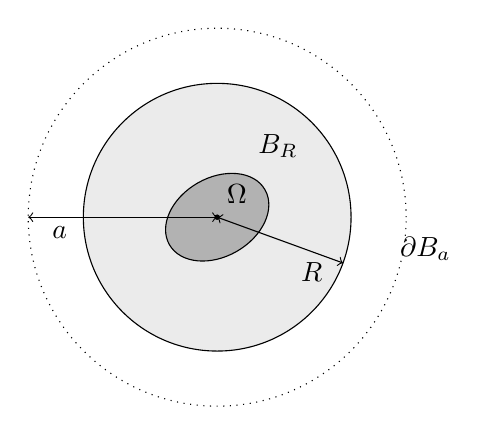
\begin{tikzpicture}
      \filldraw [fill=black!8!] (0,0)circle[radius=1.7];
      \filldraw [fill=black!30!] (-0,0)circle[x radius=0.7,y radius=0.5,rotate=30];
      \draw(0,0.3)node[right]{$\Omega$};
      \draw(0.4,0.9)node[right]{$B_R$};
      \draw(2.2,-0.4)node[right]{$\partial B_a$};
      \draw[<->](0,0)--({1.7*cos(-20)},{1.7*sin(-20)});
      \draw[<->](0,0)--(-2.4,0);
      \draw (1.2,-0.7)node{$R$};
      \draw (-2,-0.2)node{$a$};
      \fill (0,0) circle (1pt); 
      \draw[dotted] (0,0)circle[radius=2.4];
    \end{tikzpicture}
    \captionsetup[figure]{labelformat=empty,labelsep=none}
    \caption{Core-Shell Model}
  \end{figure}


\end{frame}

\begin{frame}{Core-Shell Body}

  The potential of Core-shell body $U$ is written as
  \begin{align*}
    U(x) = \underset{U^{B_R}}{\underline{\int_{B_R}E(x-y)dy}} + \rho\underset{U^{\Omega}}{\underline{\int_{\Omega}E(x-y)dy}},
  \end{align*}
  where $E$ is the fundamental solution of the Laplace equation.

  The potential $\rho U^{\Omega}$ can be calculated on the $\partial B_a$.
  \begin{align*}
    \rho U^{\Omega} = U\text{(observed)} - U^{B_R}(\text{known})\quad \mathrm{on}\quad \partial B_a.
  \end{align*}

  \begin{columns}
    \centering 
    \begin{column}{0.48\textwidth}
      \centering
      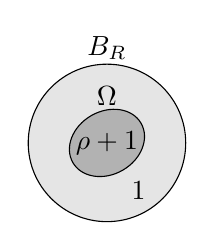
\begin{tikzpicture}
        \filldraw [fill=black!10!] (0,0)circle[radius=1.0];
        \filldraw [fill=black!30!] (-0,0)circle[x radius=0.5,y radius=0.4,rotate=30];
        \draw(0,0)node{$\rho+1$};
        \draw(0,0.6)node{$\Omega$};
        % \draw[<->](0,0)--(-0.6,0);
        % \draw[<->](0,0)--({1.6*cos(-20)},{1.6*sin(-20)});
        \draw (0.4,-0.6)node{$1$};
        \draw (0,1.2)node{$B_R$};
        % \fill (0,0) circle (1pt); 
      \end{tikzpicture}
      \captionof{figure}{Core-shell body}
    \end{column} 
    \hspace{-2cm}
    $\rightarrow$
    % \hspace{-1cm}
    \begin{column}{0.48\textwidth}
      \centering
      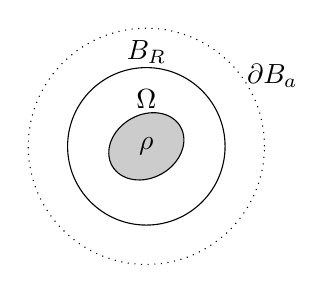
\begin{tikzpicture}
        \filldraw [fill=black!0!] (0,0)circle[radius=1.0];
        \filldraw [fill=black!20!] (-0,0)circle[x radius=0.5,y radius=0.4,rotate=30];
        \draw[dotted] (0,0)circle[radius=1.5];
        \draw(-0,0)node{$\rho$};
        \draw(0,0.6)node{$\Omega$};
        % \draw[<->](0,0)--(-0.6,0);
        % \draw[<->](0,0)--({1.6*cos(-20)},{1.6*sin(-20)});
        \draw (0,1.2)node{$B_R$};
        \draw (1.6,0.9)node{$\partial B_a$};
        % \fill (0,0) circle (1pt); 
      \end{tikzpicture}
      \captionof{figure}{Extract buried body}
    \end{column}

  \end{columns}

\end{frame}



\begin{frame}{A New Setting for The Inverse Potential Problem}
  Observe the gravity or the potential on $\partial B_a$, and recover the shape of $\Omega$.
  \begin{figure}
    \centering
    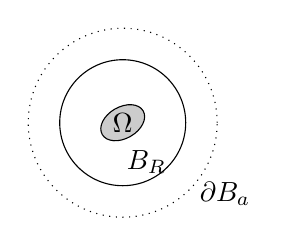
\begin{tikzpicture}
      \filldraw [fill=black!0!] (0,0)circle[radius=0.8];
      \filldraw [fill=black!20!] (-0,0)circle[x radius=0.3,y radius=0.2,rotate=30];
      \draw[dotted] (0,0)circle[radius=1.2];
      \draw(-0,0)node{$\Omega$};
      % \draw[<->](0,0)--(-0.6,0);
      % \draw[<->](0,0)--({1.6*cos(-20)},{1.6*sin(-20)});
      \draw (0.3,-0.5)node{$B_R$};
      \draw (1.3,-0.9)node{$\partial B_a$};
      % \fill (0,0) circle (1pt); 
    \end{tikzpicture}
  \end{figure}

  We will compare reconstruction by observation of the gravity and the potential.
  \begin{itemize}
    \item Observation of Gravity (traditional)
    \[
      \rho\nabla U^{\Omega} = \overrightarrow{g} \quad \mathrm{on} \quad \partial B_a
    \]
  
    \item Observation of Potential (new)
    \[
      \rho U^{\Omega} = p \quad \mathrm{on} \quad \partial B_a
    \]
  \end{itemize}
\end{frame}


\begin{frame}{Sketch of Reconstruction Algorithm}
  We can observe only at the finite points $\{A_n\}_{n=1}^N\subset\partial B_a$.
  \begin{itemize}
    \item Observation of Gravity
    \[
      \rho\nabla U^{\Omega} = \overrightarrow{g} \quad \mathrm{on} \quad \{A_n\}_{n=1}^N\subset \partial B_a
    \]
  
    \item Observation of Potential
    \[
      \rho U^{\Omega} = p \quad \mathrm{on} \quad \{A_n\}_{n=1}^N\subset \partial B_a
    \]
  \end{itemize}

  Reconstruction algorithm consists of two parts.
  \begin{enumerate}
    \item Approximate the body $\Omega$ by a set of point masses → Optimization method
    \item Homogenize the set of point masses → Bubbling method
  \end{enumerate}
  \ 
\end{frame}

\begin{frame}{Sketch of Reconstruction Algorithm}
  We can observe only at the finite points $\{A_n\}_{n=1}^N\subset\partial B_a$.
  \begin{itemize}
    \item Observation of Gravity
    \[
      \rho\nabla U^{\Omega} = \overrightarrow{g} \quad \mathrm{on} \quad \{A_n\}_{n=1}^N\subset \partial B_a
    \]
  
    \item Observation of Potential
    \[
      \rho U^{\Omega} = p \quad \mathrm{on} \quad \{A_n\}_{n=1}^N\subset \partial B_a
    \]
  \end{itemize}

  Reconstruction algorithm consists of two parts.
  \begin{enumerate}
    \item \uwave{Approximate the body $\Omega$ by a set of point masses} → Optimization method
    \item Homogenize the set of point masses → Bubbling method
  \end{enumerate}
  \ 
\end{frame}



\begin{frame}{Apprx.~Body by a Set of Point Masses (Gravity observation)}

  Observation points $\{A_n\}_{n=1}^N\subset \partial B_a$.
  \begin{figure}
    \centering
    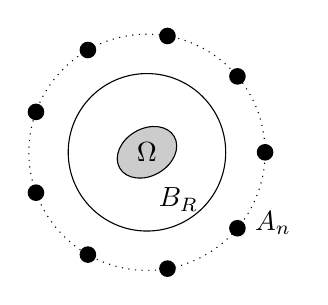
\begin{tikzpicture}
      \filldraw [fill=black!0!] (0,0)circle[radius=1.0];
      \filldraw [fill=black!20!] (-0,0)circle[x radius=0.4,y radius=0.3,rotate=30];
      \draw[dotted] (0,0)circle[radius=1.5];
      \draw(-0,0)node{$\Omega$};
      % \draw[<->](0,0)--(-0.6,0);
      % \draw[<->](0,0)--({1.6*cos(-20)},{1.6*sin(-20)});
      \draw (0.4,-0.6)node{$B_R$};
      \draw (1.6,-0.9)node{$A_n$};
      % \fill (0,0) circle (1pt); 
      \fill ({1.5*cos(0)},{1.5*sin(0}) circle (3pt); 
      \fill ({1.5*cos(40)},{1.5*sin(40}) circle (3pt); 
      \fill ({1.5*cos(80)},{1.5*sin(80}) circle (3pt); 
      \fill ({1.5*cos(120)},{1.5*sin(120}) circle (3pt); 
      \fill ({1.5*cos(160)},{1.5*sin(160}) circle (3pt); 
      \fill ({1.5*cos(200)},{1.5*sin(200)}) circle (3pt); 
      \fill ({1.5*cos(240)},{1.5*sin(240}) circle (3pt); 
      \fill ({1.5*cos(280)},{1.5*sin(280}) circle (3pt); 
      \fill ({1.5*cos(320)},{1.5*sin(320}) circle (3pt); 
    \end{tikzpicture}
  \end{figure}

  We difine a cost function $J_G$ as following.
  set of point mass has representation $(X,M)=(X_1,\dots X_K, M_1,\dots M_K)$.
  \begin{gather*}
    J_G(X, M) = \frac{1}{N}\sum_{n=1}^N\left|\rho\nabla U^{\Omega}(A_n) - G_K(A_n;X,M)\right|^2,\\ 
    \quad G_K(A_n;X,M) = \frac{1}{4\pi}\sum_{k=1}^K\frac{M_k(A_n-X_k)}{|A_n-X_k|^3}
  \end{gather*}
\end{frame}

\begin{frame}{Apprx.~Body by a Set of Point Mass (Potential observation)}
  Observation points $\{A_n\}_{n=1}^N\subset \partial B_a$.
  \begin{figure}
    \centering
    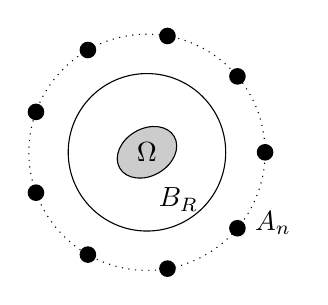
\begin{tikzpicture}
      \filldraw [fill=black!0!] (0,0)circle[radius=1.0];
      \filldraw [fill=black!20!] (-0,0)circle[x radius=0.4,y radius=0.3,rotate=30];
      \draw[dotted] (0,0)circle[radius=1.5];
      \draw(-0,0)node{$\Omega$};
      % \draw[<->](0,0)--(-0.6,0);
      % \draw[<->](0,0)--({1.6*cos(-20)},{1.6*sin(-20)});
      \draw (0.4,-0.6)node{$B_R$};
      \draw (1.6,-0.9)node{$A_n$};
      % \fill (0,0) circle (1pt); 
      \fill ({1.5*cos(0)},{1.5*sin(0}) circle (3pt); 
      \fill ({1.5*cos(40)},{1.5*sin(40}) circle (3pt); 
      \fill ({1.5*cos(80)},{1.5*sin(80}) circle (3pt); 
      \fill ({1.5*cos(120)},{1.5*sin(120}) circle (3pt); 
      \fill ({1.5*cos(160)},{1.5*sin(160}) circle (3pt); 
      \fill ({1.5*cos(200)},{1.5*sin(200)}) circle (3pt); 
      \fill ({1.5*cos(240)},{1.5*sin(240}) circle (3pt); 
      \fill ({1.5*cos(280)},{1.5*sin(280}) circle (3pt); 
      \fill ({1.5*cos(320)},{1.5*sin(320}) circle (3pt); 
    \end{tikzpicture}
  \end{figure}

  We difine a cost function $J_P$ as following.
  set of point mass has representation $(X,M)=(X_1,\dots X_K, M_1,\dots M_K)$.
  \begin{gather*}
    J_P(X, M) = \frac{1}{N}\sum_{n=1}^N\left|\rho U^{\Omega}(A_n) - P_K(A_n;X,M)\right|^2, \\
    P_K(A_n;X,M) = \frac{1}{4\pi}\sum_{k=1}^K \frac{M_k}{|A_n-X_k|}
  \end{gather*}
\end{frame}

\begin{frame}{Sketch of Reconstruction Algorithm}
  We can observe only at the finite points $\{A_n\}_{n=1}^N\subset\partial B_a$.
  \begin{itemize}
    \item Observation of Gravity
    \[
      \rho\nabla U^{\Omega} = \overrightarrow{g} \quad \mathrm{on} \quad \{A_n\}_{n=1}^N\subset \partial B_a
    \]
  
    \item Observation of Potential
    \[
      \rho U^{\Omega} = p \quad \mathrm{on} \quad \{A_n\}_{n=1}^N\subset \partial B_a
    \]
  \end{itemize}

  Reconstruction algorithm consists of two parts.
  \begin{enumerate}
    \item Approximate the body $\Omega$ by a set of point masses → Optimization method
    \item \uwave{Homogenize the set of point masses} → Bubbling method
  \end{enumerate}
  \ 
\end{frame}




\begin{frame}{Bubbling Method (Partial Mass Scattering)}
  We homogenize the set of point masses to homogeneous body with density $\rho$.

  Point mass $(X_k,M_k)$ move to lattice point $\widetilde{X}_k=(ih, jh)$.

  $\widetilde{M}_{i,j}=M_k$.
  When $\Delta \widetilde{M}_{i,j} = \widetilde{M}_{i,j}-\rho h^2 > \varepsilon$,
  \begin{gather*}
    \widetilde{M}_{i,j}^{(1)}=\rho h^2-\varepsilon, \\
    \widetilde{M}_{i\pm 1,j}^{(1)}=\widetilde{M}_{i\pm 1,j}+\frac{1}{4}(\Delta \widetilde{M}_{i,j}+\varepsilon),\quad
    \widetilde{M}_{i,j\pm 1}^{(1)}=\widetilde{M}_{i,j\pm 1}+\frac{1}{4}(\Delta \widetilde{M}_{i,j}+\varepsilon).
  \end{gather*}
  \begin{columns}
    \centering 
    \begin{column}{0.48\textwidth}
      \centering
        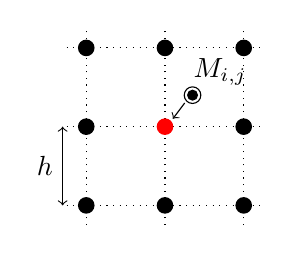
\begin{tikzpicture}
          \draw [dotted,thin] (-1.25,-1.25) grid [step=1] (1.25,1.25);
          \fill [red] (0,0) circle (3pt); 
          \draw (0.35,0.40) circle (3pt); 
          \fill (0.35,0.40) circle (2pt); 

          \fill (1,0) circle (3pt);
          \fill (1,1) circle (3pt);
          \fill (0,1) circle (3pt);
          \fill (-1,1) circle (3pt);
          \fill (-1,0) circle (3pt);
          \fill (-1,-1) circle (3pt);
          \fill (0,-1) circle (3pt);
          \fill (1,-1) circle (3pt);

          \draw[<->](-1.3,-1)--(-1.3,0);
          \node[left] at (-1.3,-0.5){$h$};

          \draw(0.7,0.7)node{$M_{i,j}$};
          \draw[->](0.25,0.30)--(0.1,0.1);
        \end{tikzpicture}
        \captionof{figure}{Move to lattice point}
    \end{column} 
    \hspace{-1cm}

    \hspace{-1cm}
    \begin{column}{0.48\textwidth}
      \centering
        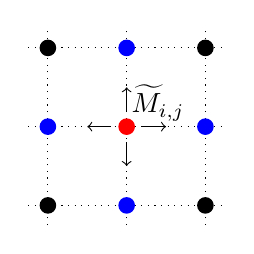
\begin{tikzpicture}
          \draw [dotted,thin] (-1.25,-1.25) grid [step=1] (1.25,1.25);
          \fill [red] (0,0) circle (3pt); 
          \fill [blue] (-1,0) circle (3pt); 
          \fill [blue] (1,0) circle (3pt); 
          \fill [blue] (0,1) circle (3pt); 
          \fill [blue] (0,-1) circle (3pt); 

          \fill (1,1) circle (3pt); 
          \fill (1,-1) circle (3pt); 
          \fill (-1,1) circle (3pt); 
          \fill (-1,-1) circle (3pt); 

          \draw(0.4,0.3)node{$\widetilde{M}_{i,j}$};
          \draw[->](0.2,0)--(0.5,0);
          \draw[->](0,0.2)--(0,0.5);
          \draw[->](-0.2,0)--(-0.5,0);
          \draw[->](0,-0.2)--(0,-0.5);
        \end{tikzpicture}
        \captionof{figure}{Mass Scattering}
    \end{column}

  \end{columns}


\end{frame}

% \begin{frame}{数値計算 バブリング法の設定}
  % 格子点$(ih,jh)$に乗っている質量を$\widetilde{M}_{i,j}$で表す.
  % $\Delta \widetilde{M}_{i,j} = \widetilde{M}_{i,j}-\rho h^2 > \varepsilon$とき,
  % \[
    % \widetilde{M}_{i,j}^{(1)}=\rho h^2-\varepsilon
  % \]
  % で更新する.
  % メッシュ幅$h$は$10^{-2}$,パラメータ$\varepsilon$は$10^{-5}$とした.
  % \begin{figure}
    % \begin{tikzpicture}
      % \draw [dotted,thin] (-2.2,-2.2) grid (2.2,2.2);
      % \fill (-2,2) circle (3pt); 
      % \fill (-1,2) circle (3pt); 
      % \fill (0,2) circle (3pt); 
      % \fill (1,2) circle (3pt); 
      % \fill (2,2) circle (3pt); 

      % \fill (-2,1) circle (3pt); 
      % \fill (-1,1) circle (3pt); 
      % \fill (0,1) circle (3pt); 
      % \fill (1,1) circle (3pt); 
      % \fill (2,1) circle (3pt); 

      % \fill (-2,0) circle (3pt); 
      % \fill (-1,0) circle (3pt); 
      % \fill (0,0) circle (3pt); 
      % \fill (1,0) circle (3pt); 
      % \fill (2,0) circle (3pt); 

      % \fill (-2,-1) circle (3pt); 
      % \fill (-1,-1) circle (3pt); 
      % \fill (0,-1) circle (3pt); 
      % \fill (1,-1) circle (3pt); 
      % \fill (2,-1) circle (3pt); 

      % \fill (-2,-2) circle (3pt); 
      % \fill (-1,-2) circle (3pt); 
      % \fill (0,-2) circle (3pt); 
      % \fill (1,-2) circle (3pt); 
      % \fill (2,-2) circle (3pt); 

      % % \draw (1.8,1.3) circle (3pt); 
      % % \fill (1.8,1.3) circle (2pt); 

      % \fill [red] (2,1) circle (3pt); 
      % \fill [red] (-1,-1) circle (3pt); 

      % \fill [blue] (-2,-1) circle (3pt); 
      % \fill [blue] (-1,-2) circle (3pt); 
      % \fill [blue] (-1,0) circle (3pt); 
      % \fill [blue] (0,-1) circle (3pt); 

      % \fill [blue] (1,1) circle (3pt); 
      % \fill [blue] (2,0) circle (3pt); 
      % \fill [blue] (2,2) circle (3pt); 
      % % \fill [blue] (3,1) circle (3pt); 

      % \draw[->](-0.8,-1)--(-0.2,-1);
      % \draw[->](-1.2,-1)--(-1.8,-1);
      % \draw[->](-1,-0.8)--(-1,-0.2);
      % \draw[->](-1,-1.2)--(-1,-1.8);

      % \draw[-](2.2,1)--(2.4,1);
      % \draw[->](1.8,1)--(1.2,1);
      % \draw[->](2,1.2)--(2,1.8);
      % \draw[->](2,0.8)--(2,0.2);
    % \end{tikzpicture}
    % \caption{バブリング法}
  % \end{figure}
% \end{frame}

\begin{frame}{Reconfirm The Aid of Computation} 
  When we change radius of observation $a$, 
  we verify influence for the reconstruction which is caused by this change.

  \begin{figure}
    \centering
    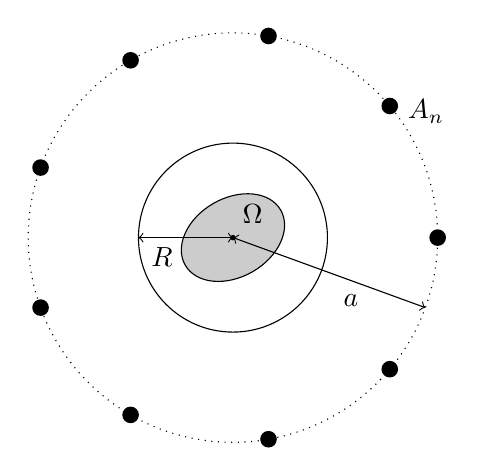
\begin{tikzpicture}
      \filldraw [fill=black!20!] (-0,0)circle[x radius=0.7,y radius=0.5,rotate=30];
      \draw(0,0.3)node[right]{$\Omega$};
      \draw(2.1,1.6)node[right]{$A_n$};
      \draw[<->](0,0)--(-1.2,0);
      \draw[<->](0,0)--({2.6*cos(-20)},{2.6*sin(-20)});
      \draw (-0.9,0)node[below]{$R$};
      \draw (1.5,-0.8)node{$a$};
      \fill (0,0) circle (1pt); 
      \draw (0,0)circle[radius=1.2];
      \draw[dotted] (0,0)circle[radius=2.6];

      \fill ({2.6*cos(0)},{2.6*sin(0}) circle (3pt); 
      \fill ({2.6*cos(40)},{2.6*sin(40}) circle (3pt); 
      \fill ({2.6*cos(80)},{2.6*sin(80}) circle (3pt); 
      \fill ({2.6*cos(120)},{2.6*sin(120}) circle (3pt); 
      \fill ({2.6*cos(160)},{2.6*sin(160}) circle (3pt); 
      \fill ({2.6*cos(200)},{2.6*sin(200)}) circle (3pt); 
      \fill ({2.6*cos(240)},{2.6*sin(240}) circle (3pt); 
      \fill ({2.6*cos(280)},{2.6*sin(280}) circle (3pt); 
      \fill ({2.6*cos(320)},{2.6*sin(320}) circle (3pt); 
    \end{tikzpicture}
    \captionsetup[figure]{labelformat=empty,labelsep=none}
    \caption{Observation at $\{A_n\}_{n=1}^N$ and Reconstruction $\Omega\subset B_R$}
  \end{figure}

\end{frame}




% \begin{frame}{円板の回復}
  % 原点中心半径$1$の円板の回復を試みる.

  % 質点の数$K=1$,観測点$N=3$とし,観測半径$R$を変えてその影響について数値計算する.
  % 最適化にはNewton法を用いた.
  % コスト関数$J_P, J_G$を$0$とする$(X_1,M_1)$が存在し,いずれの場合も$X_1=0, M_1=\pi$に限られている.

  % \begin{figure}
    % \centering
    % \begin{tikzpicture}
      % \filldraw [fill=black!10!] (0,0) circle [radius=0.5];
      % \fill (0,0) circle (1pt); 
      % \draw[dotted] (0,0)circle[radius=1];
      % \draw[<->](0,0)--(-1,0);
      % \draw[<->](0,0)--({2*cos(-20)},{2*sin(-20)});
      % \draw(1.5,0)node[below]{$R$};
      % \draw(-0.7,0)node[above]{$r_0$};
      % \draw (0,0)circle[radius=2];
      % \fill (2,0) circle (3pt); 
      % \fill ({2*cos(0)},{2*sin(0}) circle (3pt); 
      % \fill ({2*cos(120)},{2*sin(120}) circle (3pt); 
      % \fill ({2*cos(240)},{2*sin(240}) circle (3pt); 
    % \end{tikzpicture}
  % \end{figure}

% \end{frame}



\begin{frame}{Example: Reconstruction of Ellipzoid}
  Set $R=2$.
  We reconstruct an elliptic shape with long radius $\sqrt{2}$, short radius $1$ and density $\rho=10$.
  Limit of resolution is $10^{-4}$.

  We select Levenberg-Marquardt method as a optimization method.

  \begin{figure}
    \centering
    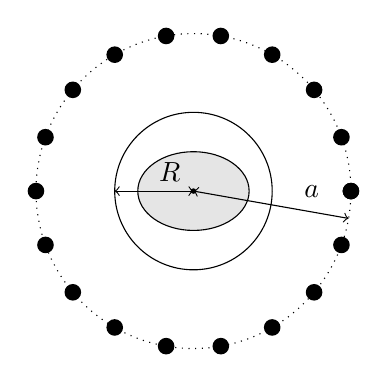
\begin{tikzpicture}
      % \filldraw[fill=black!10!] ({-0.25*sqrt(3)},-0.25) -- ++(0:{0.5*sqrt(3)}) -- ++(120:{0.5*sqrt(3)}) -- cycle;
      \filldraw [fill=black!10!] (0,0)circle[x radius=0.707,y radius=0.5,rotate=0];
      \fill (0,0) circle (1pt); 
      \draw (0,0)circle[radius=1];
      \draw[<->](0,0)--(-1,0);
      \draw[<->](0,0)--({2*cos(-10)},{2*sin(-10)});
      \draw(1.5,0)node{$a$};
      \draw(-0.3,0)node[above]{$R$};
      \draw[dotted] (0,0)circle[radius=2];
      \fill (2,0) circle (3pt); 
      \fill ({2*cos(0)},{2*sin(0}) circle (3pt); 
      \fill ({2*cos(20)},{2*sin(20}) circle (3pt); 
      \fill ({2*cos(40)},{2*sin(40}) circle (3pt); 
      \fill ({2*cos(60)},{2*sin(60}) circle (3pt); 
      \fill ({2*cos(80)},{2*sin(80}) circle (3pt); 
      \fill ({2*cos(100)},{2*sin(100}) circle (3pt); 
      \fill ({2*cos(120)},{2*sin(120}) circle (3pt); 
      \fill ({2*cos(140)},{2*sin(140}) circle (3pt); 
      \fill ({2*cos(160)},{2*sin(160}) circle (3pt); 
      \fill ({2*cos(180)},{2*sin(180}) circle (3pt); 
      \fill ({2*cos(200)},{2*sin(200}) circle (3pt); 
      \fill ({2*cos(220)},{2*sin(220}) circle (3pt); 
      \fill ({2*cos(240)},{2*sin(240}) circle (3pt); 
      \fill ({2*cos(260)},{2*sin(260}) circle (3pt); 
      \fill ({2*cos(280)},{2*sin(280}) circle (3pt); 
      \fill ({2*cos(300)},{2*sin(300}) circle (3pt); 
      \fill ({2*cos(320)},{2*sin(320}) circle (3pt); 
      \fill ({2*cos(340)},{2*sin(340}) circle (3pt); 
    \end{tikzpicture}
  \end{figure}

\end{frame}

\begin{frame}{Example: Observation of Gravity}
  Number of point masses is $K=100$, number of observation points is $N=300$.
  $a$ is observation radius.

  \begin{columns}
    \begin{column}{0.38\columnwidth}
      \centering
      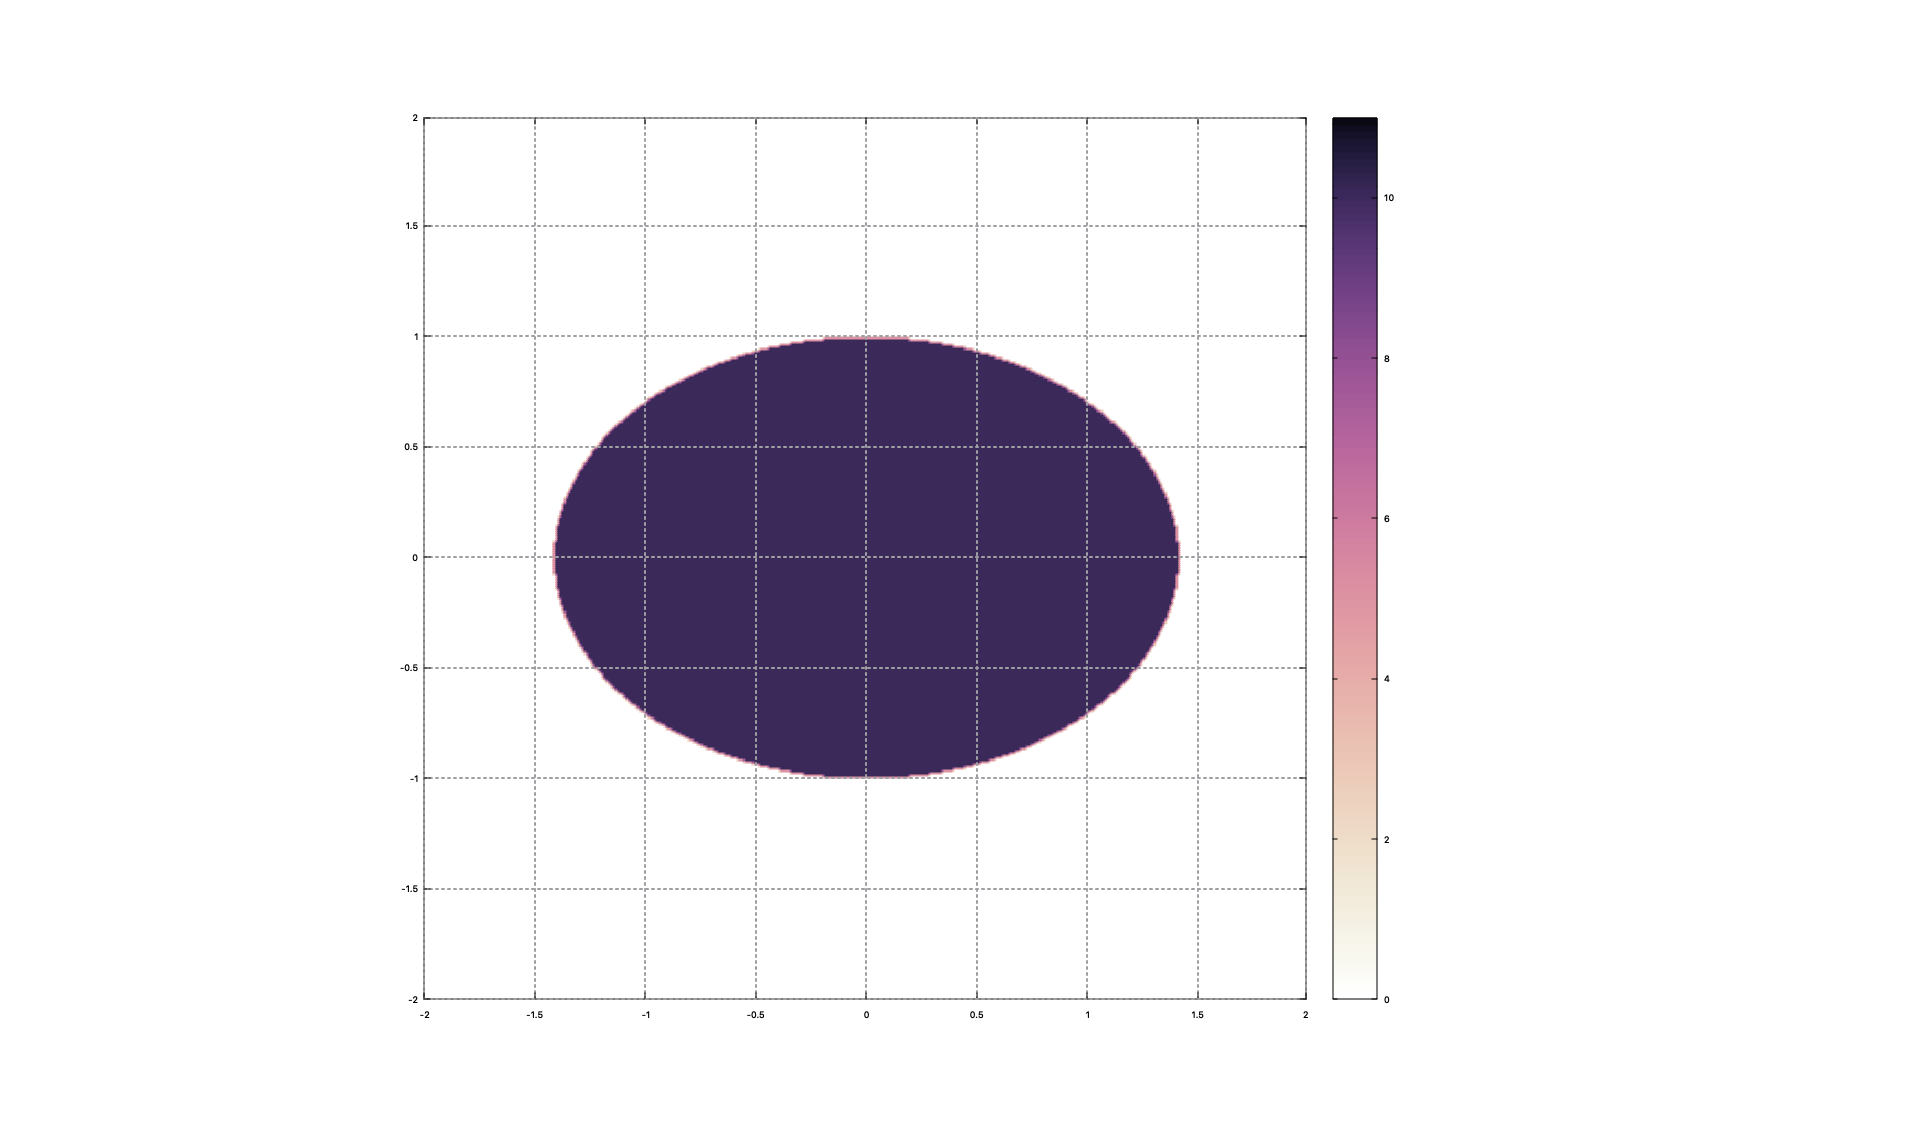
\includegraphics[width=4cm]{fig/elliptic.png}
      \captionsetup[figure]{labelformat=empty,labelsep=none}
      \captionof{figure}{source}
    \end{column}
    \hspace{-1cm}
    \begin{column}{0.38\columnwidth}
      \centering
      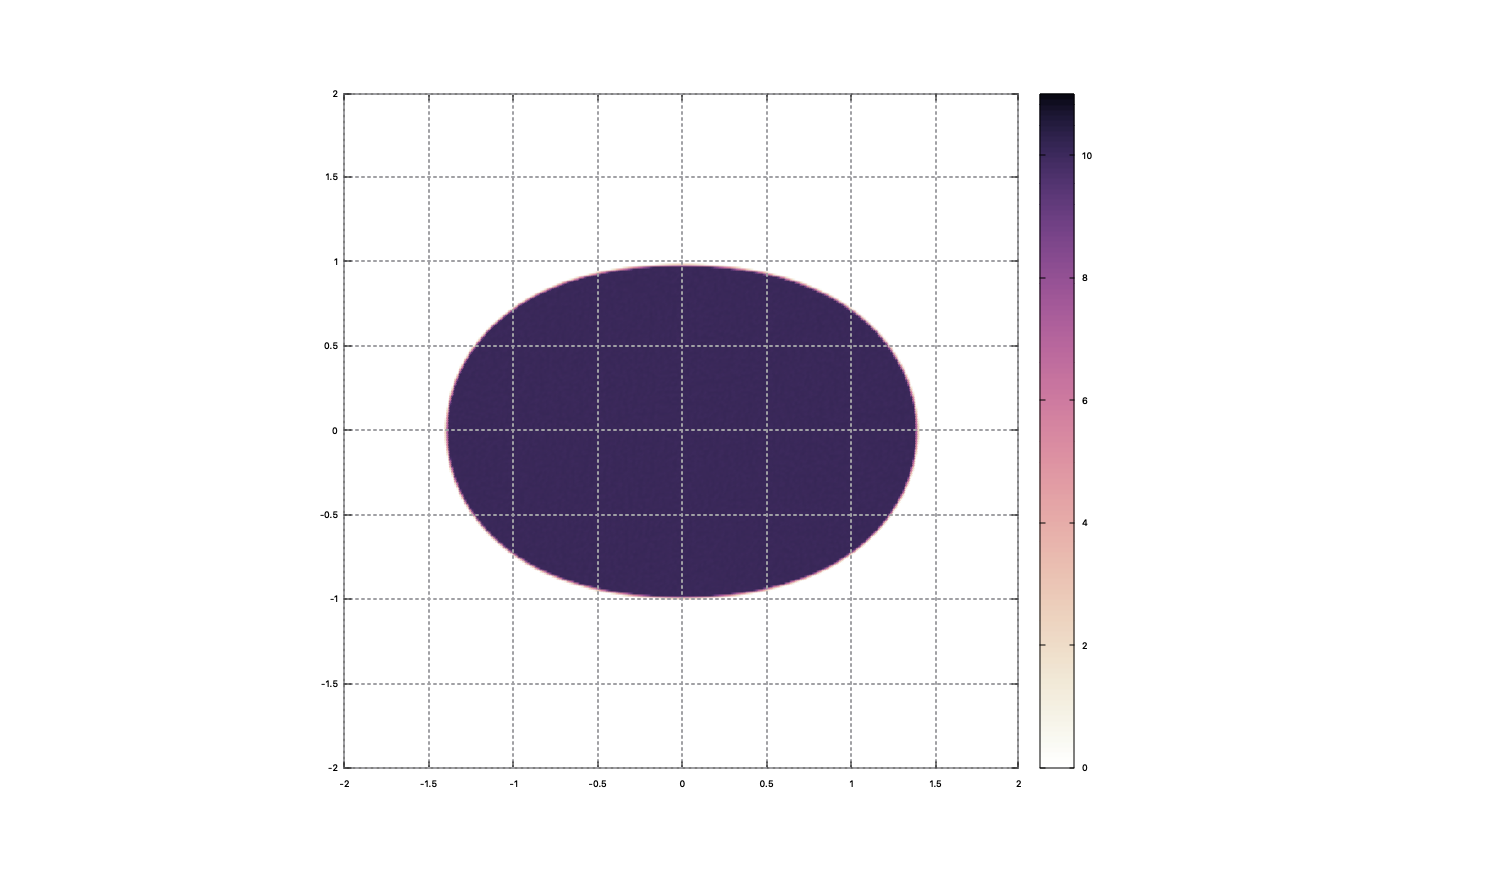
\includegraphics[width=4cm]{fig2/GN300K100R10E2.png}
      \captionsetup[figure]{labelformat=empty,labelsep=none}
      \captionof{figure}{$a=10$}
    \end{column}
  \end{columns}

  \begin{columns}
    \begin{column}{0.38\columnwidth}
      \centering
      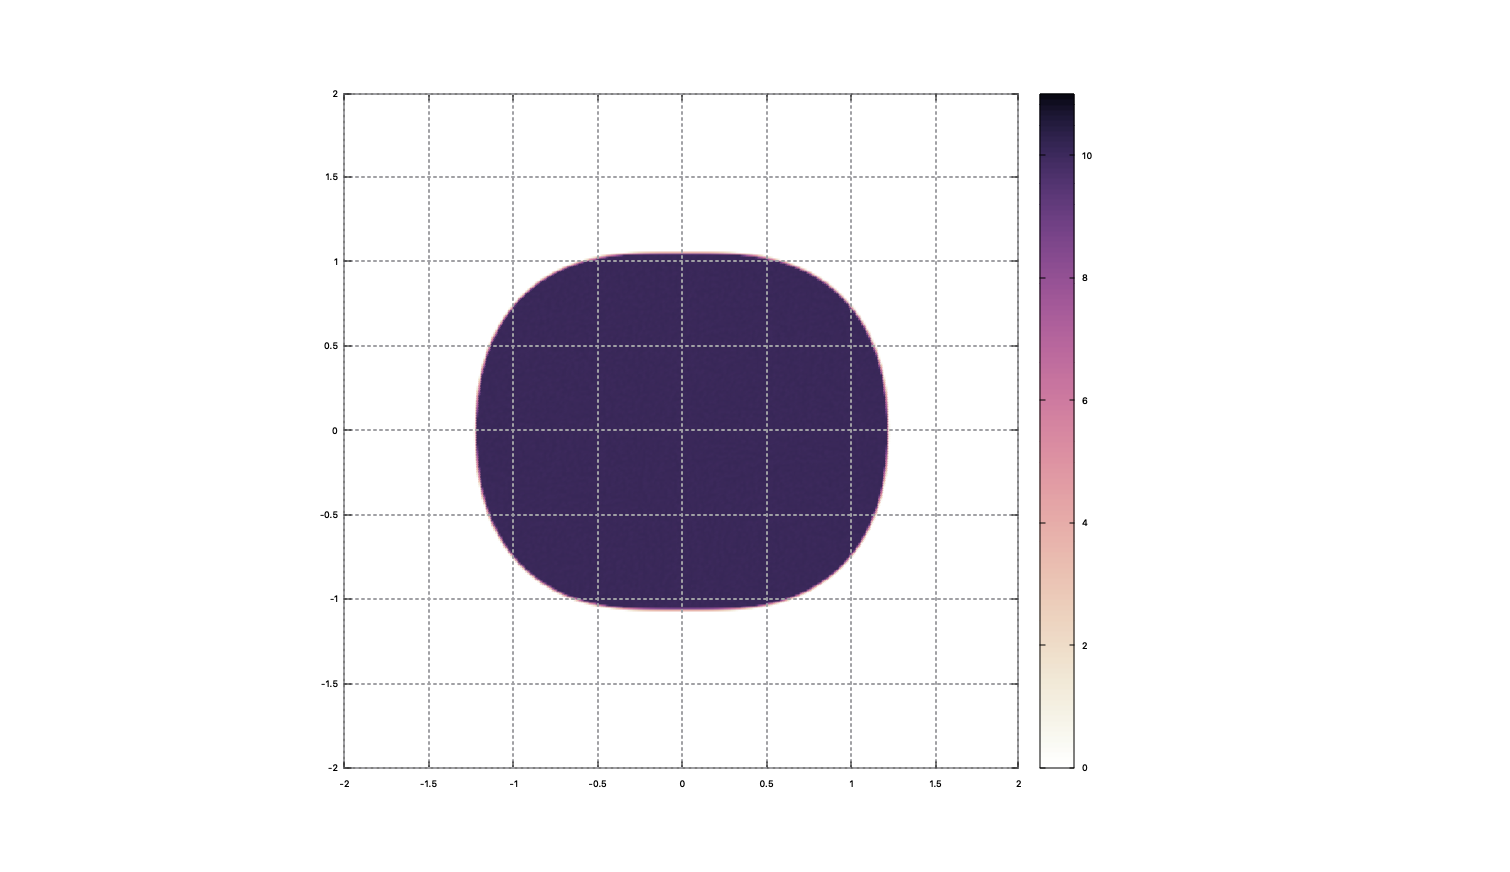
\includegraphics[width=4cm]{fig2/GN300K100R30E2.png}
      \captionsetup[figure]{labelformat=empty,labelsep=none}
      \captionof{figure}{$a=30$}
    \end{column}
    \hspace{-1cm}
    \begin{column}{0.38\columnwidth}
      \centering
      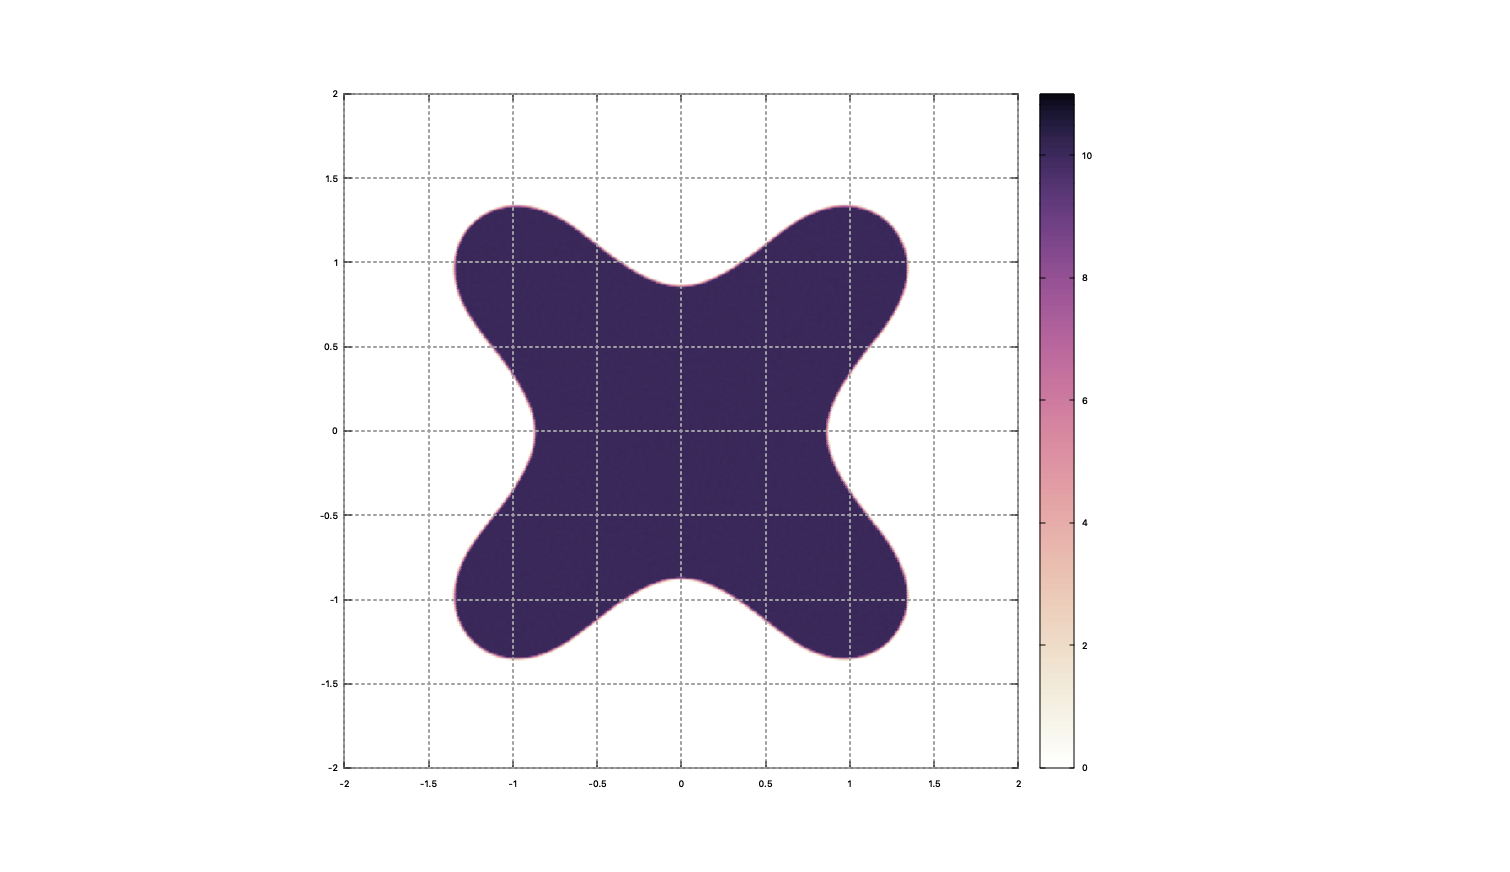
\includegraphics[width=4cm]{fig3/GN300K100R200E2.png}
      \captionsetup[figure]{labelformat=empty,labelsep=none}
      \captionof{figure}{$a=200$}
    \end{column}
  \end{columns}


\end{frame}

\begin{frame}{Example: Observation of Potential}
  Number of point masses is $K=100$, number of observation points is $N=300$.
  $a$ is observation radius.

  \begin{columns}
    \begin{column}{0.38\columnwidth}
      \setcounter{figure}{5}
      \centering
      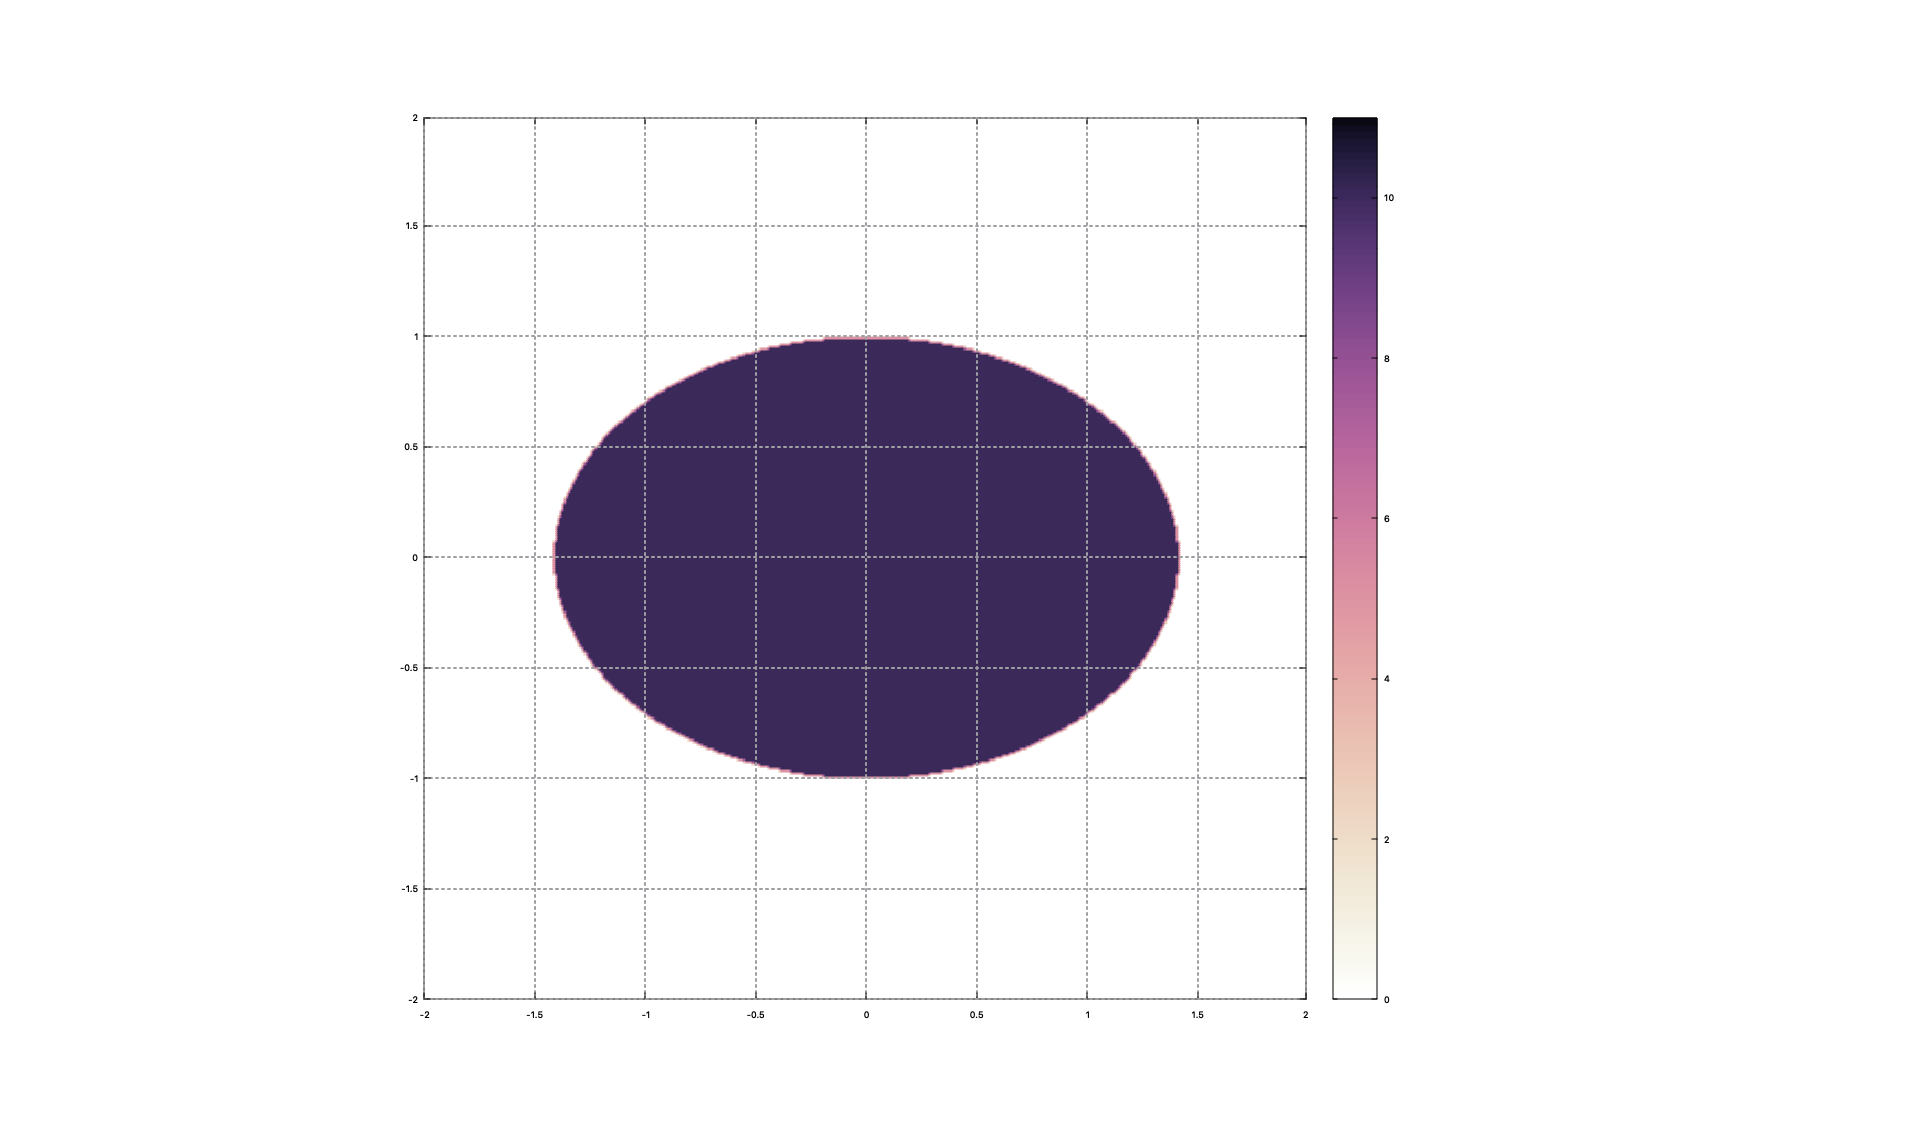
\includegraphics[width=4cm]{fig/elliptic.png}
      \captionsetup[figure]{labelformat=empty,labelsep=none}
      \captionof{figure}{source}
    \end{column}
    \hspace{-1cm}
    \begin{column}{0.38\columnwidth}
      \setcounter{figure}{9}
      \centering
      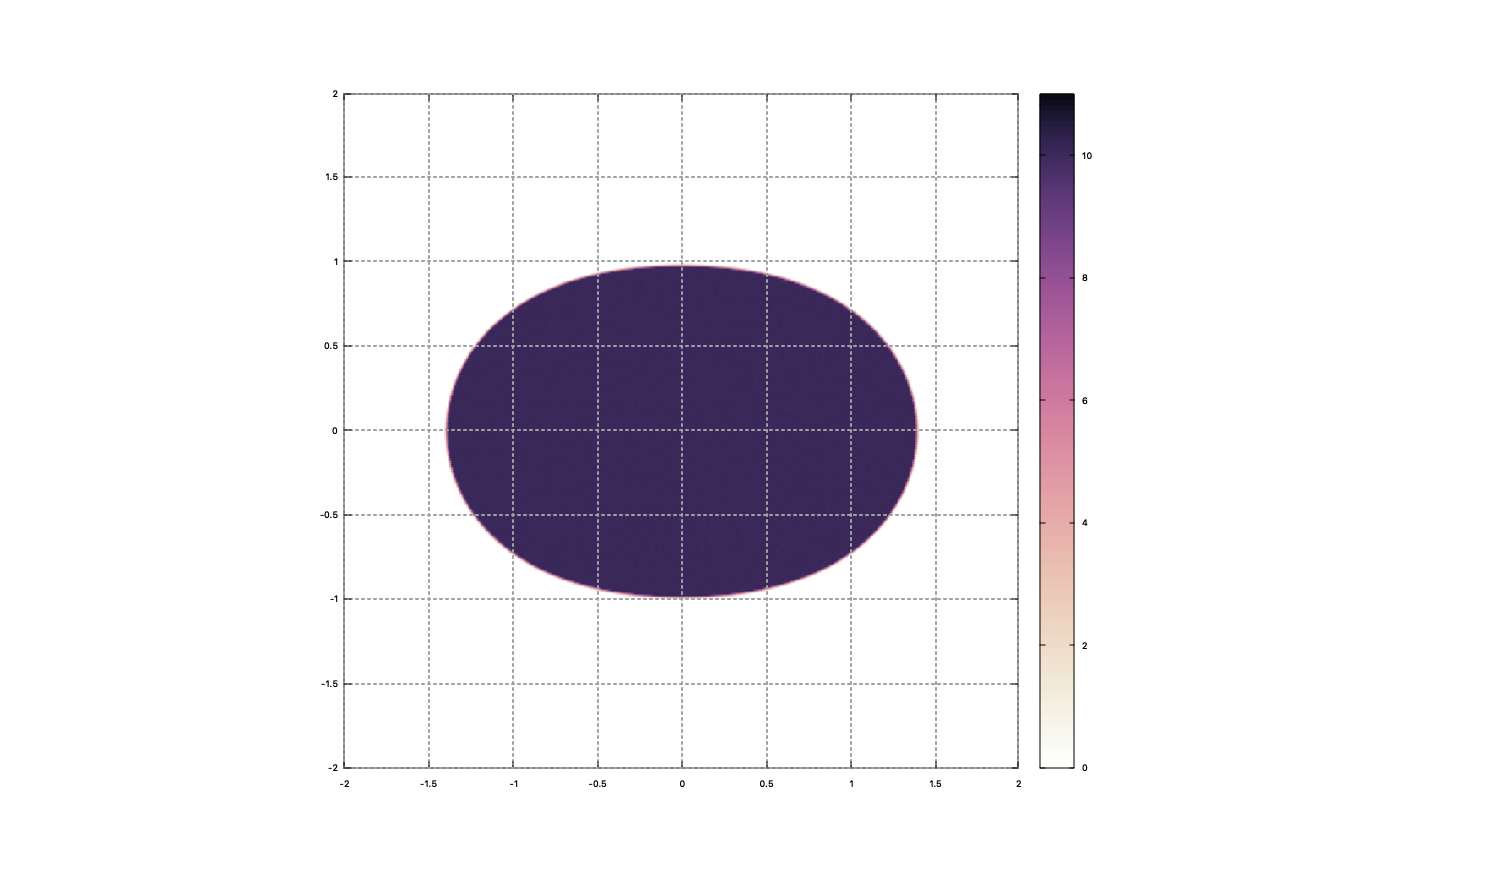
\includegraphics[width=4cm]{fig2/PN300K100R10E2.png}
      \captionsetup[figure]{labelformat=empty,labelsep=none}
      \captionof{figure}{$a=10$}
    \end{column}
  \end{columns}

  \begin{columns}
    \begin{column}{0.38\columnwidth}
      \centering
      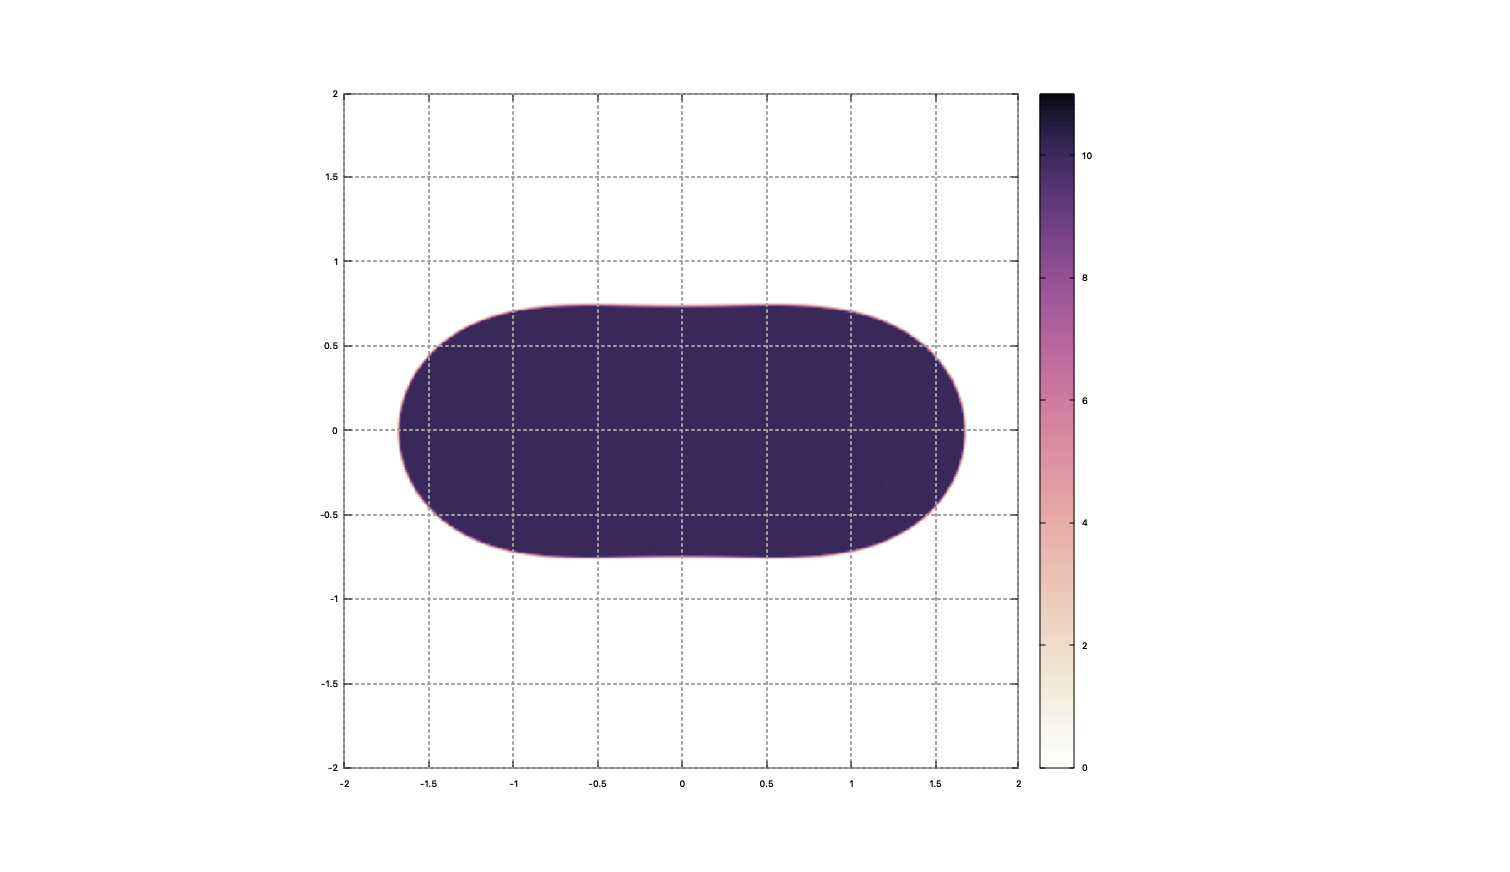
\includegraphics[width=4cm]{fig2/PN300K100R30E2.png}
      \captionsetup[figure]{labelformat=empty,labelsep=none}
      \captionof{figure}{$a=30$}
    \end{column}
    \hspace{-1cm}
    \begin{column}{0.38\columnwidth}
      \centering
      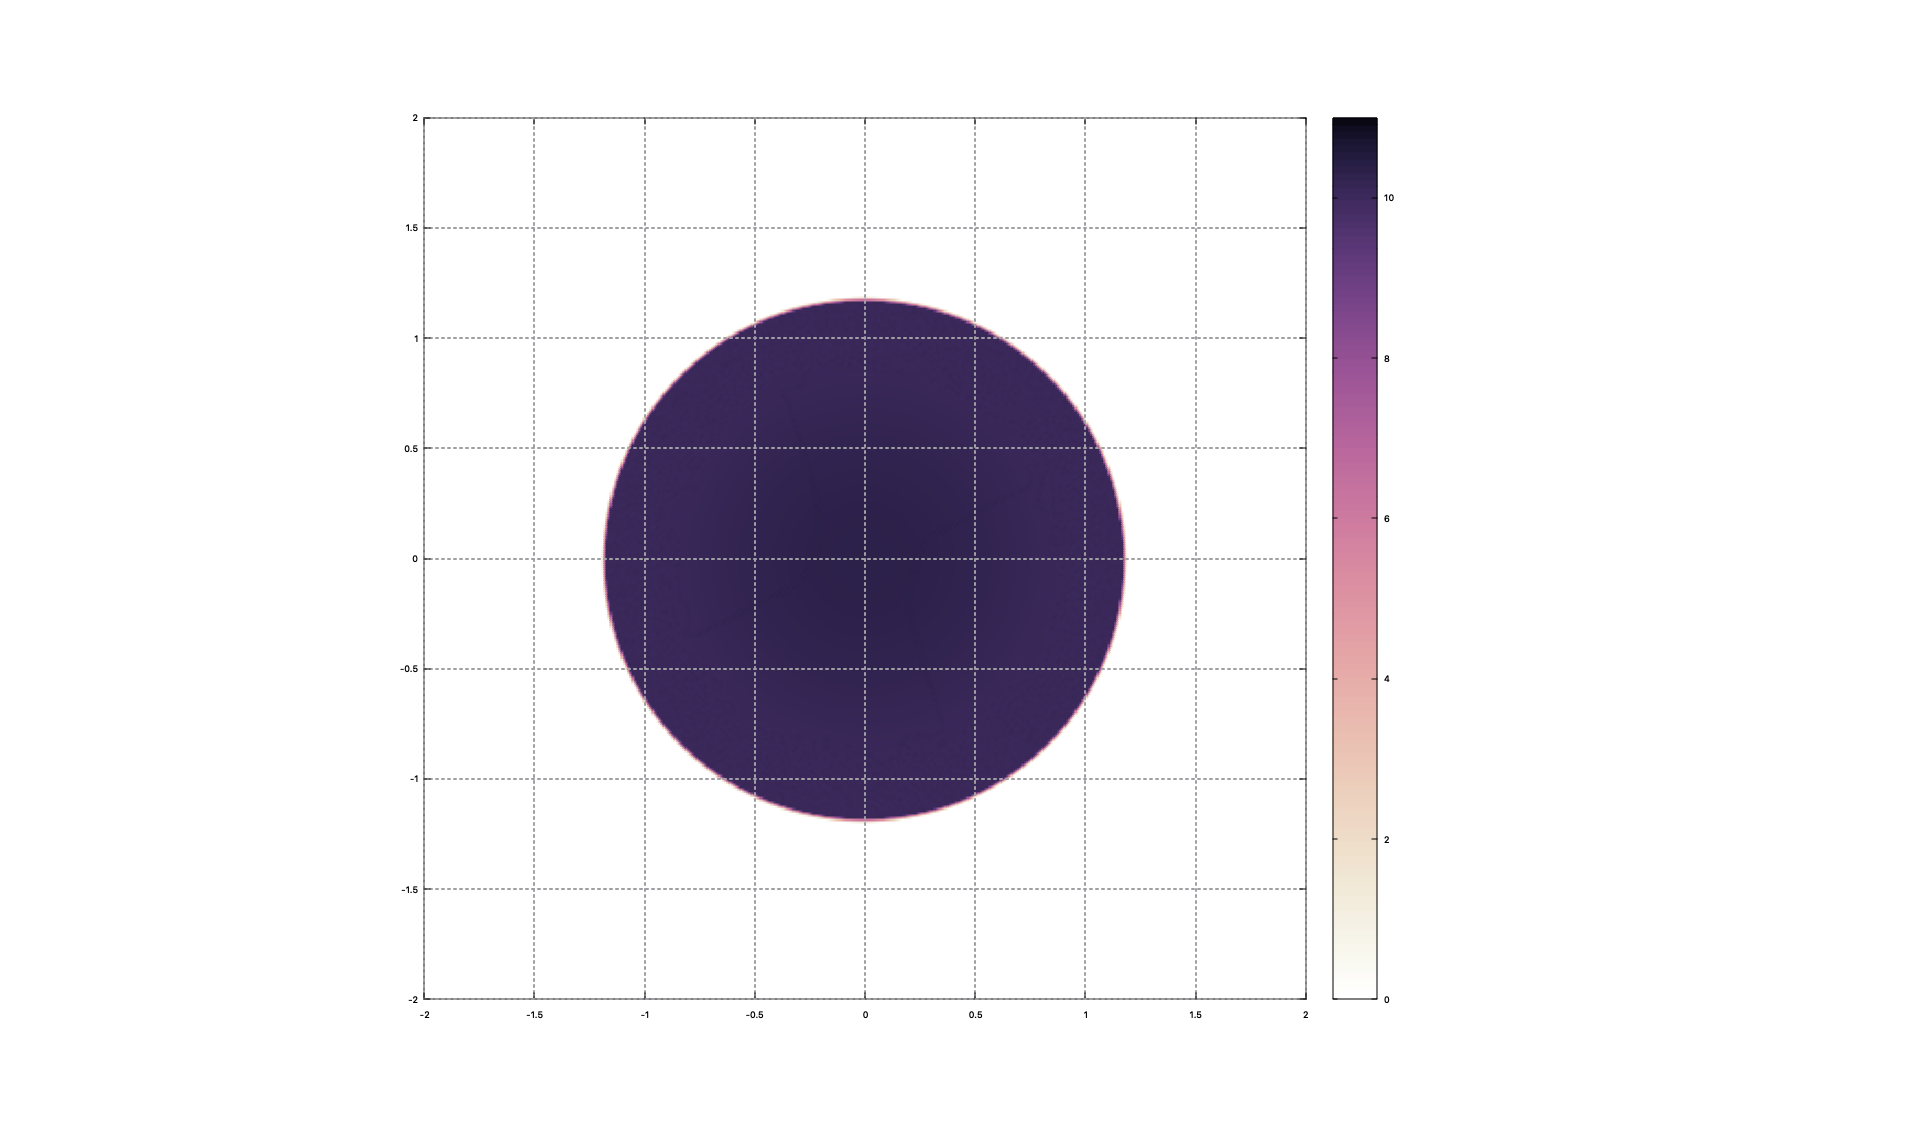
\includegraphics[width=4cm]{fig3/PN300K100R200E2.png}
      \captionsetup[figure]{labelformat=empty,labelsep=none}
      \captionof{figure}{$a=200$}
    \end{column}
  \end{columns}

\end{frame}


\begin{frame}{Conclusion}

  We observe the potential and reconstruct the shape of the body, compared to observation of the gravity.

  \begin{itemize}

    \item Reconstruction of Ellipzoid

    Reconstruction by observation of the potential can reconstruct source body more correctly.

  \end{itemize}

  \begin{figure}
    \centering
    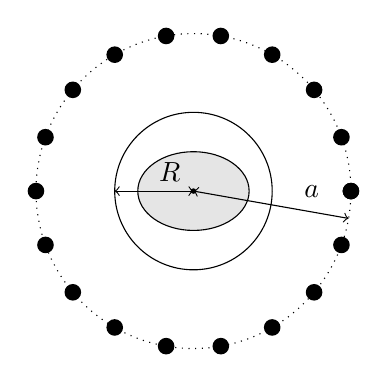
\begin{tikzpicture}
      % \filldraw[fill=black!10!] ({-0.25*sqrt(3)},-0.25) -- ++(0:{0.5*sqrt(3)}) -- ++(120:{0.5*sqrt(3)}) -- cycle;
      \filldraw [fill=black!10!] (0,0)circle[x radius=0.707,y radius=0.5,rotate=0];
      \fill (0,0) circle (1pt); 
      \draw (0,0)circle[radius=1];
      \draw[<->](0,0)--(-1,0);
      \draw[<->](0,0)--({2*cos(-10)},{2*sin(-10)});
      \draw(1.5,0)node{$a$};
      \draw(-0.3,0)node[above]{$R$};
      \draw[dotted] (0,0)circle[radius=2];
      \fill (2,0) circle (3pt); 
      \fill ({2*cos(0)},{2*sin(0}) circle (3pt); 
      \fill ({2*cos(20)},{2*sin(20}) circle (3pt); 
      \fill ({2*cos(40)},{2*sin(40}) circle (3pt); 
      \fill ({2*cos(60)},{2*sin(60}) circle (3pt); 
      \fill ({2*cos(80)},{2*sin(80}) circle (3pt); 
      \fill ({2*cos(100)},{2*sin(100}) circle (3pt); 
      \fill ({2*cos(120)},{2*sin(120}) circle (3pt); 
      \fill ({2*cos(140)},{2*sin(140}) circle (3pt); 
      \fill ({2*cos(160)},{2*sin(160}) circle (3pt); 
      \fill ({2*cos(180)},{2*sin(180}) circle (3pt); 
      \fill ({2*cos(200)},{2*sin(200}) circle (3pt); 
      \fill ({2*cos(220)},{2*sin(220}) circle (3pt); 
      \fill ({2*cos(240)},{2*sin(240}) circle (3pt); 
      \fill ({2*cos(260)},{2*sin(260}) circle (3pt); 
      \fill ({2*cos(280)},{2*sin(280}) circle (3pt); 
      \fill ({2*cos(300)},{2*sin(300}) circle (3pt); 
      \fill ({2*cos(320)},{2*sin(320}) circle (3pt); 
      \fill ({2*cos(340)},{2*sin(340}) circle (3pt); 
    \end{tikzpicture}
  \end{figure}


\end{frame}

% \begin{frame}[noframenumbering]{付録:初期値依存}
  % 質点数$K=100$,観測点数$N=300$とする.
  % $a$は観測半径である.

  % \begin{columns}
    % \begin{column}{0.38\columnwidth}
      % \centering
      % 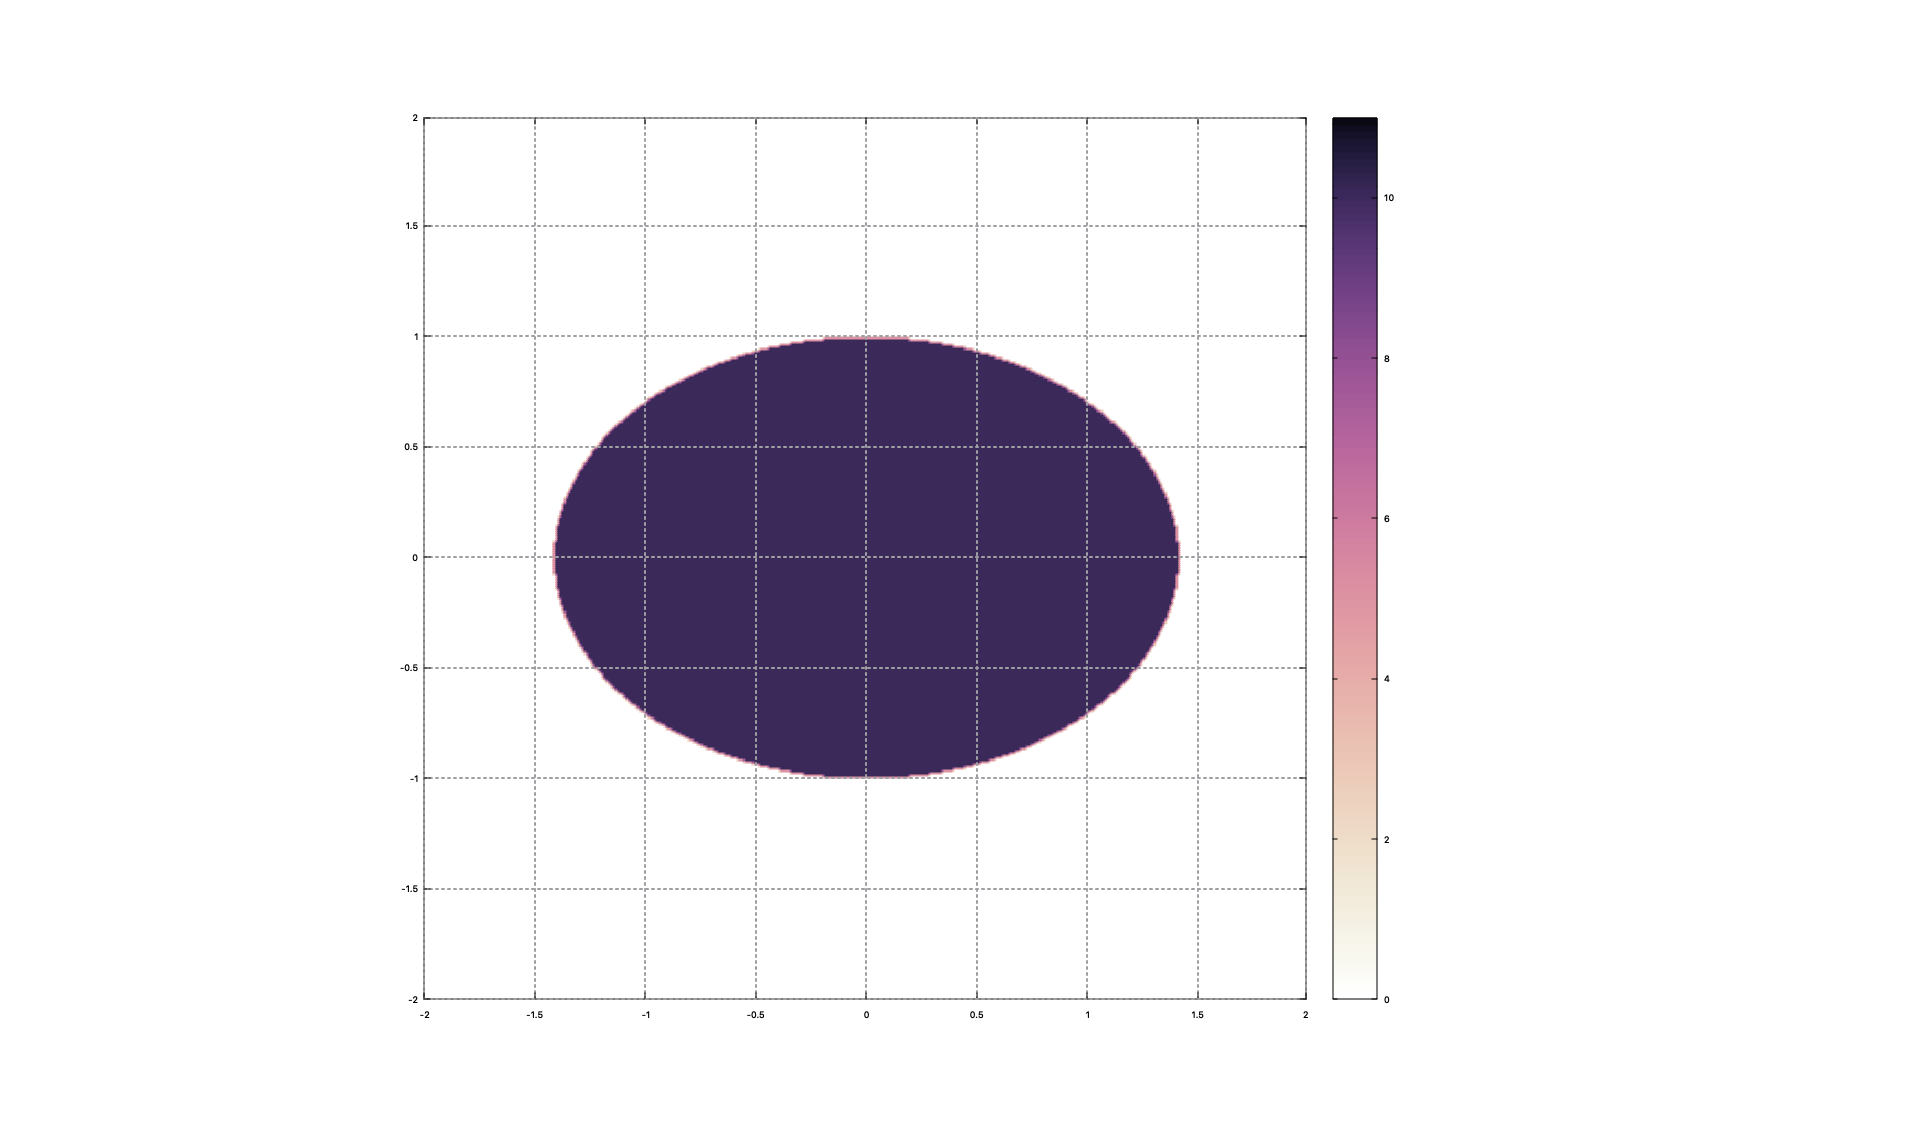
\includegraphics[width=4cm]{fig/elliptic.png}
      % \captionsetup[figure]{labelformat=empty,labelsep=none}
      % \captionof{figure}{厳密解}
    % \end{column}
    % \hspace{-1cm}
    % \begin{column}{0.38\columnwidth}
      % \centering
      % 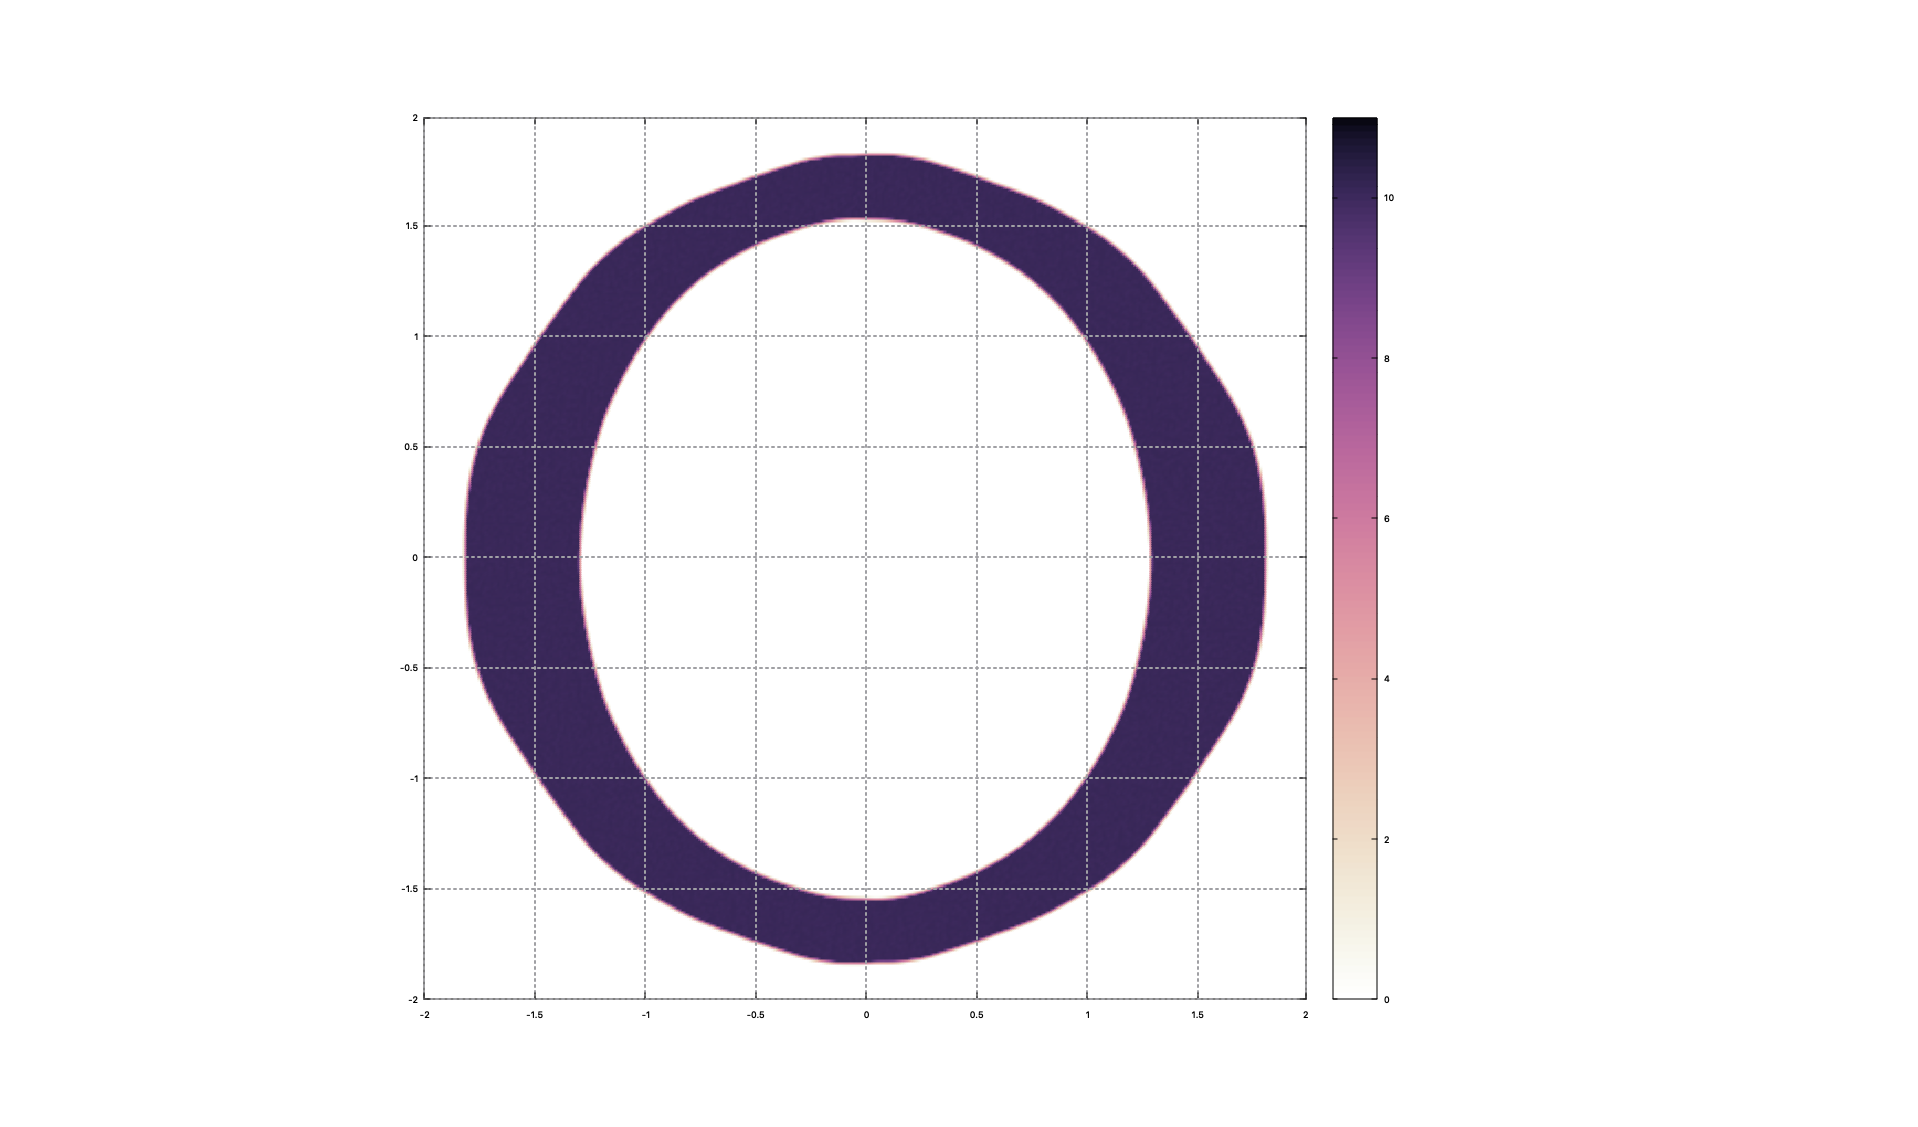
\includegraphics[width=4cm]{fig/GN300K100R4E2.png}
      % \captionsetup[figure]{labelformat=empty,labelsep=none}
      % \captionof{figure}{$a=4$}
    % \end{column}
  % \end{columns}

  % \begin{columns}
    % \begin{column}{0.38\columnwidth}
      % \centering
      % 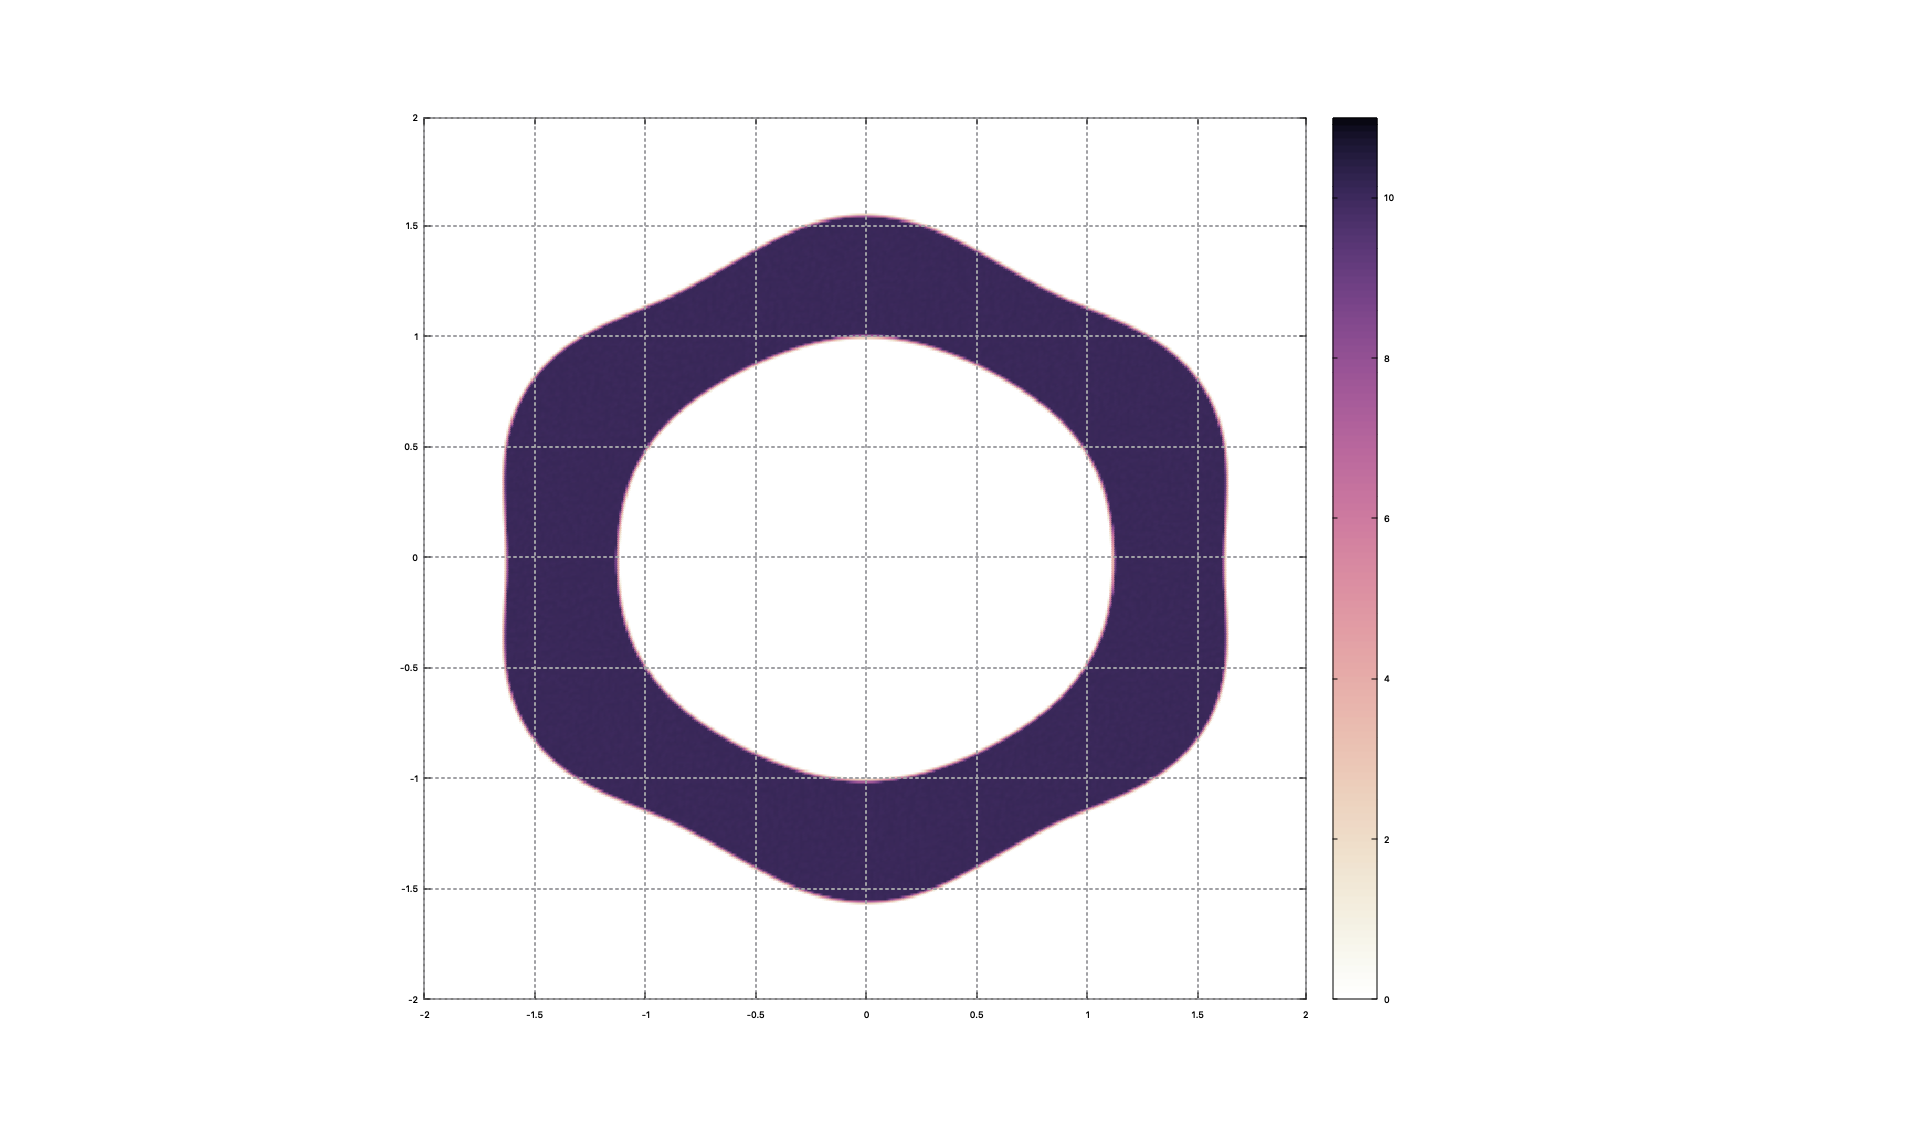
\includegraphics[width=4cm]{fig/GN300K100R10E2.png}
      % \captionsetup[figure]{labelformat=empty,labelsep=none}
      % \captionof{figure}{$a=10$}
    % \end{column}
    % \hspace{-1cm}
    % \begin{column}{0.38\columnwidth}
      % \centering
      % 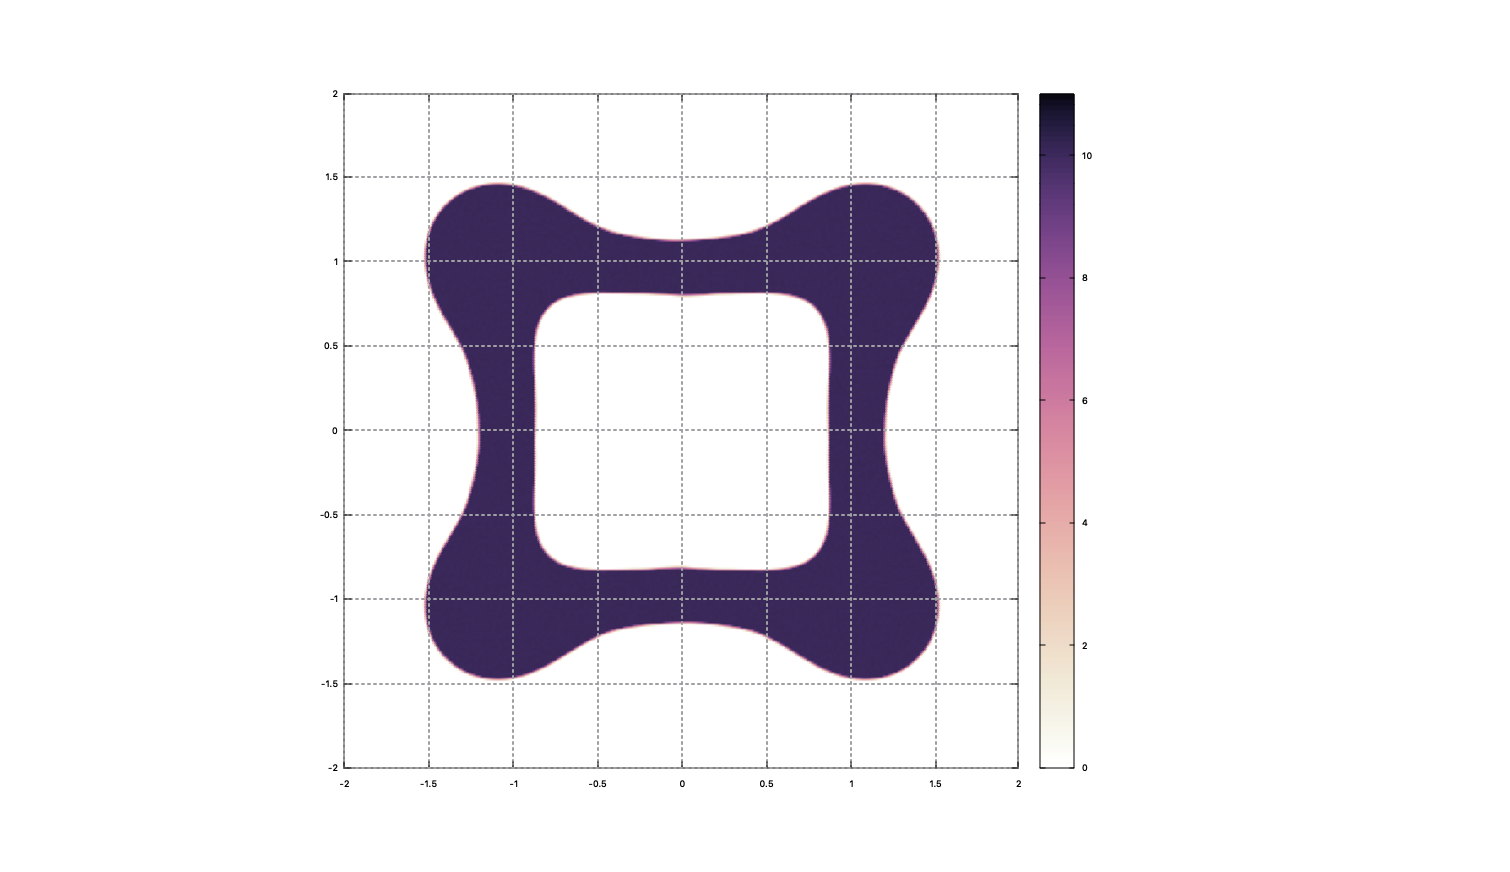
\includegraphics[width=4cm]{fig/GN300K100R30E2.png}
      % \captionsetup[figure]{labelformat=empty,labelsep=none}
      % \captionof{figure}{$a=30$}
    % \end{column}
  % \end{columns}


% \end{frame}

% \begin{frame}[noframenumbering]{付録:初期値依存}
  % 質点数$K=100$,観測点数$N=300$とする.
  % $a$は観測半径である.

  % \begin{columns}
    % \begin{column}{0.38\columnwidth}
      % \setcounter{figure}{5}
      % \centering
      % 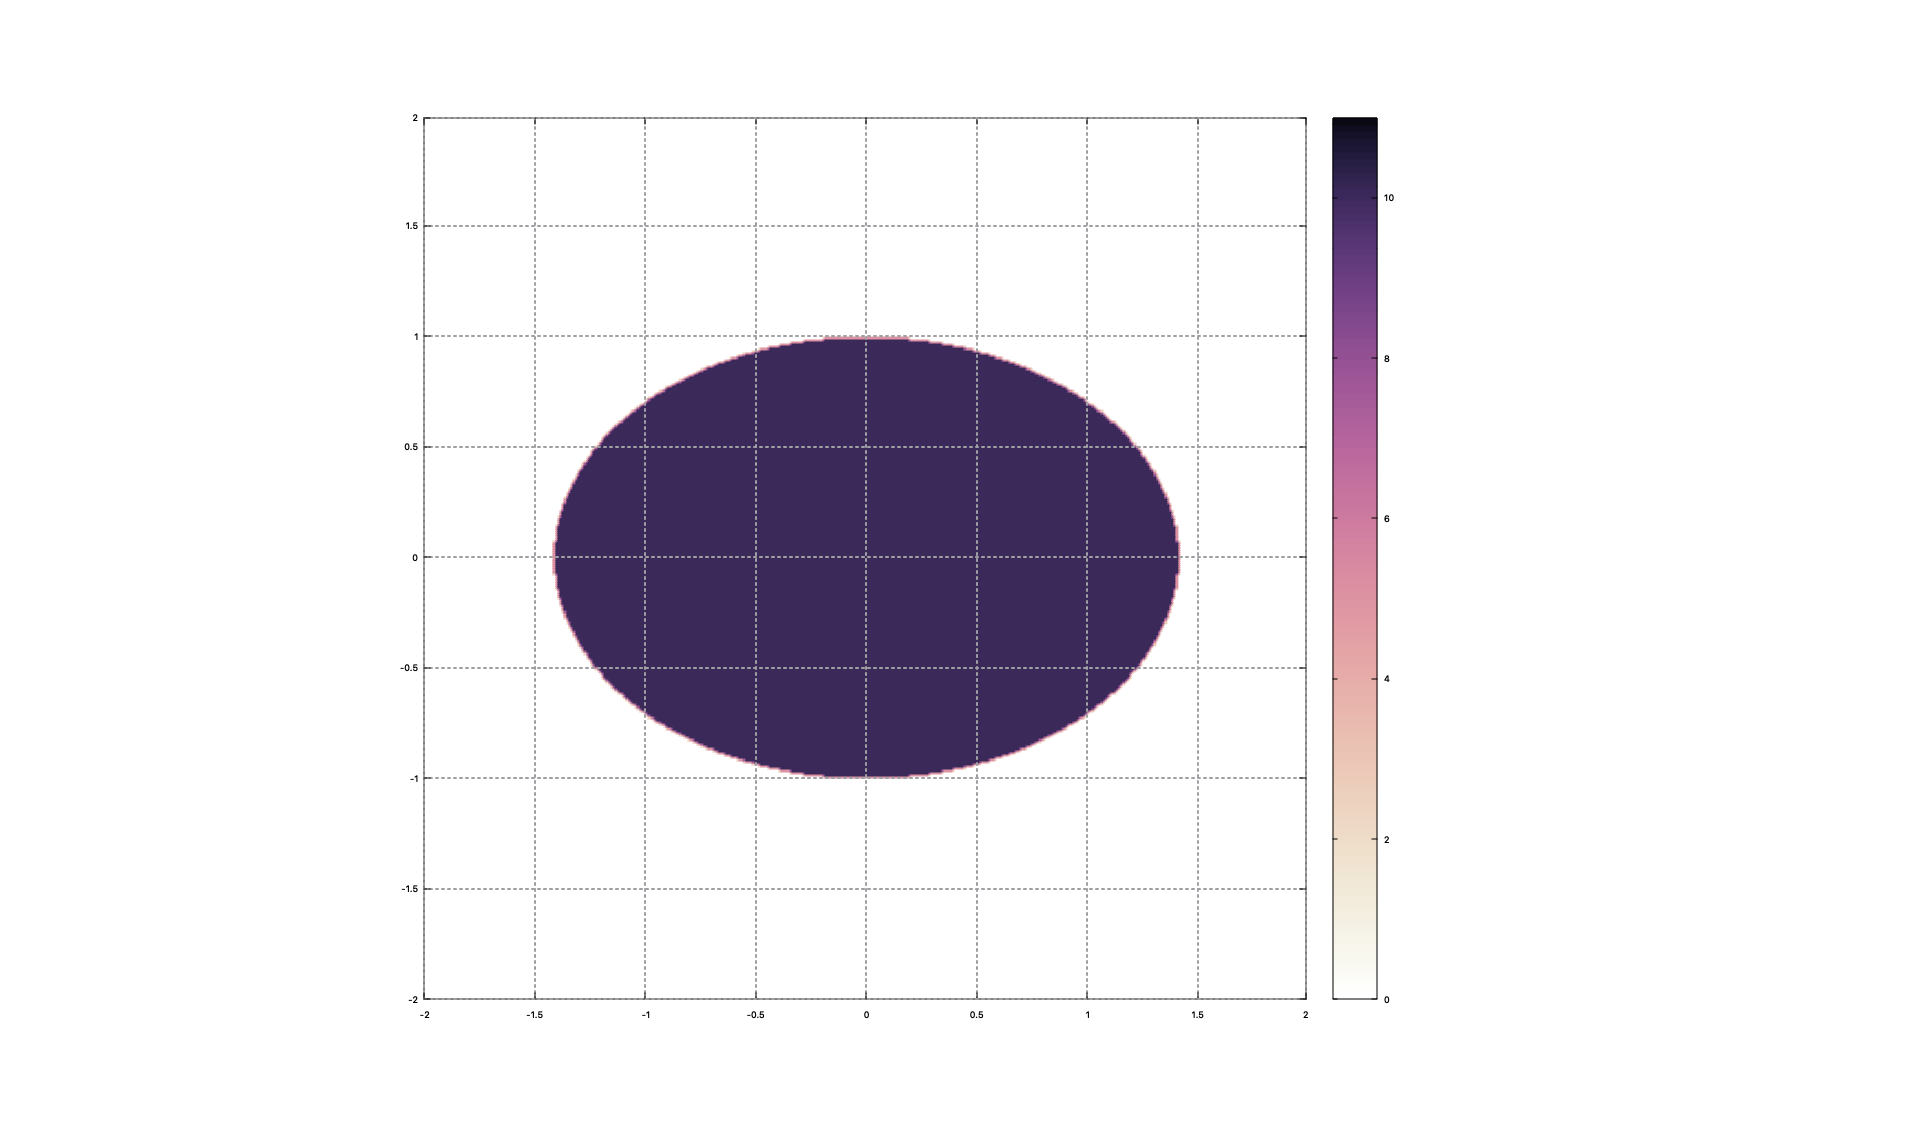
\includegraphics[width=4cm]{fig/elliptic.png}
      % \captionsetup[figure]{labelformat=empty,labelsep=none}
      % \captionof{figure}{厳密解}
    % \end{column}
    % \hspace{-1cm}
    % \begin{column}{0.38\columnwidth}
      % \setcounter{figure}{9}
      % \centering
      % 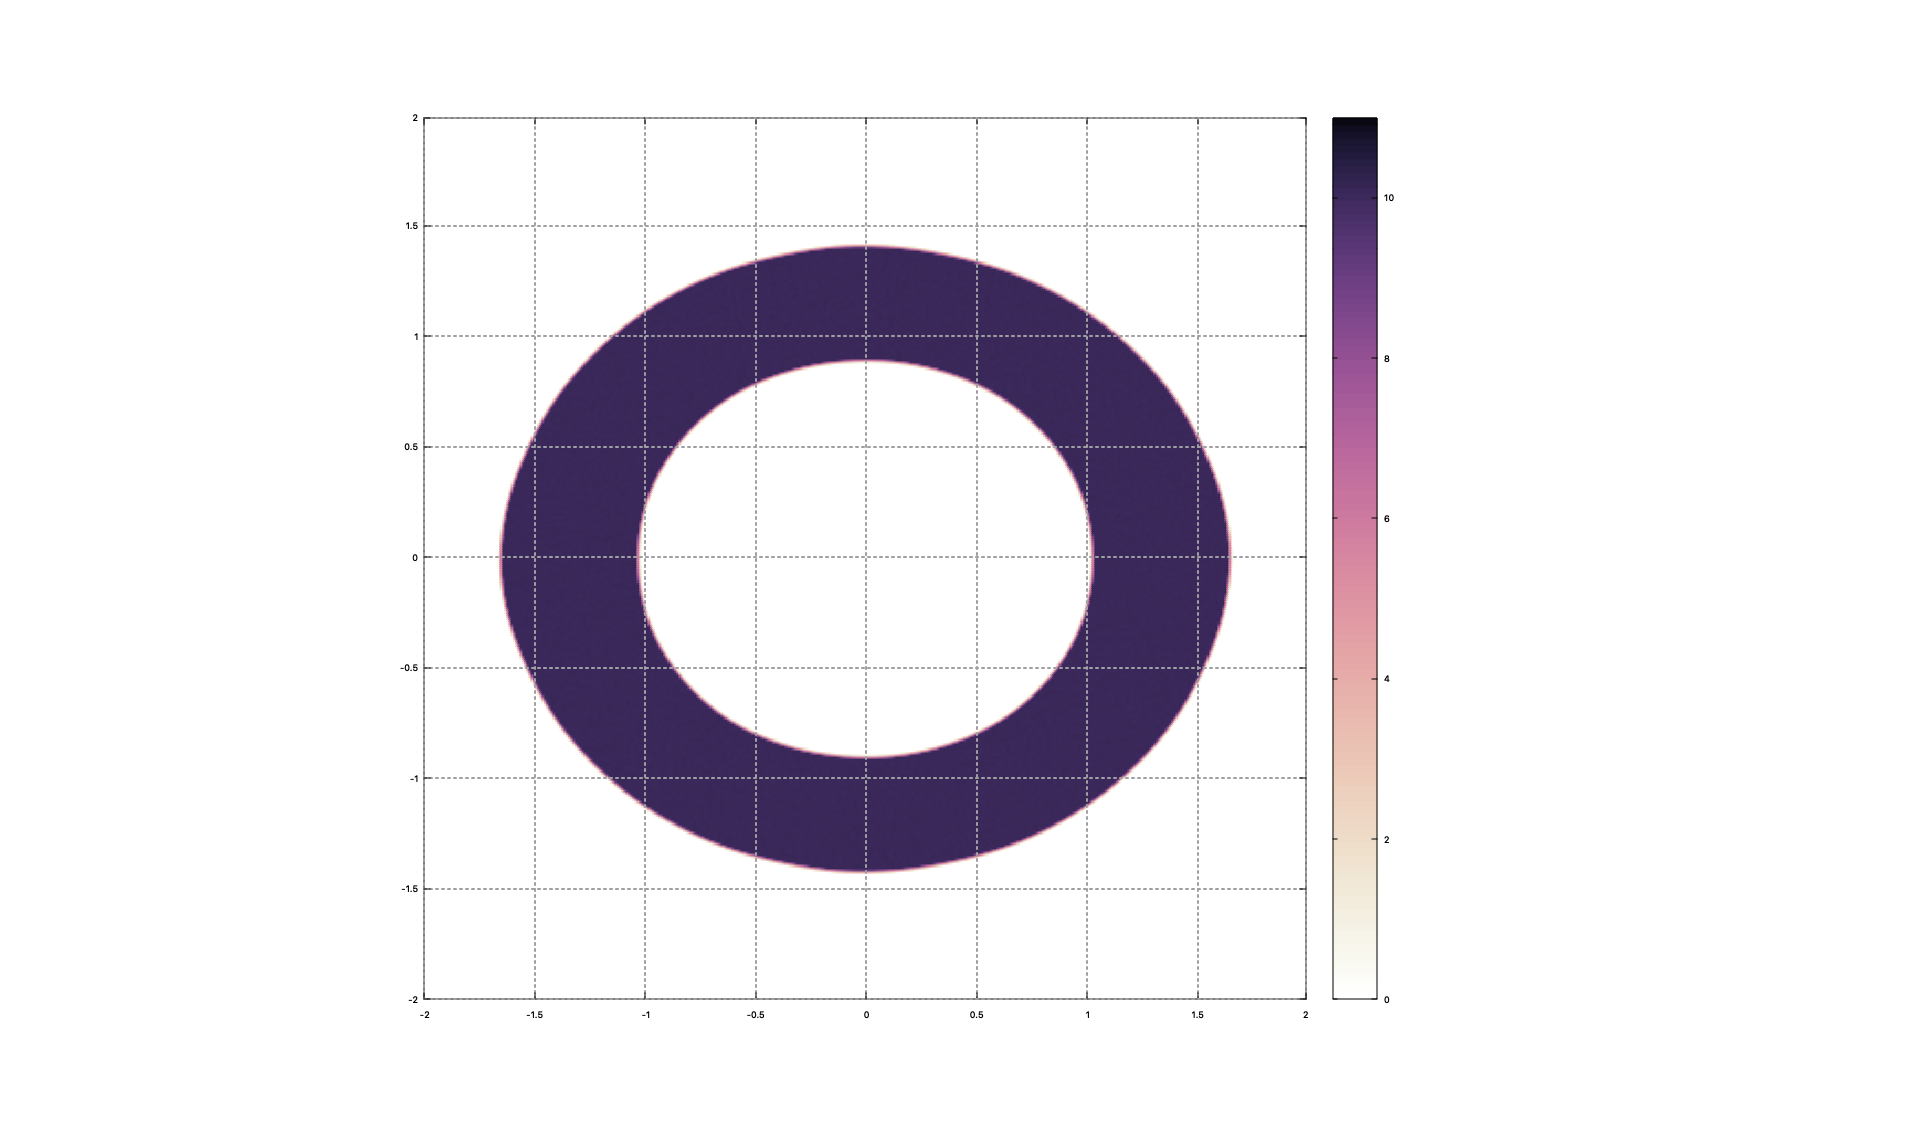
\includegraphics[width=4cm]{fig/PN300K100R4E2.png}
      % \captionsetup[figure]{labelformat=empty,labelsep=none}
      % \captionof{figure}{$a=4$}
    % \end{column}
  % \end{columns}

  % \begin{columns}
    % \begin{column}{0.38\columnwidth}
      % \centering
      % 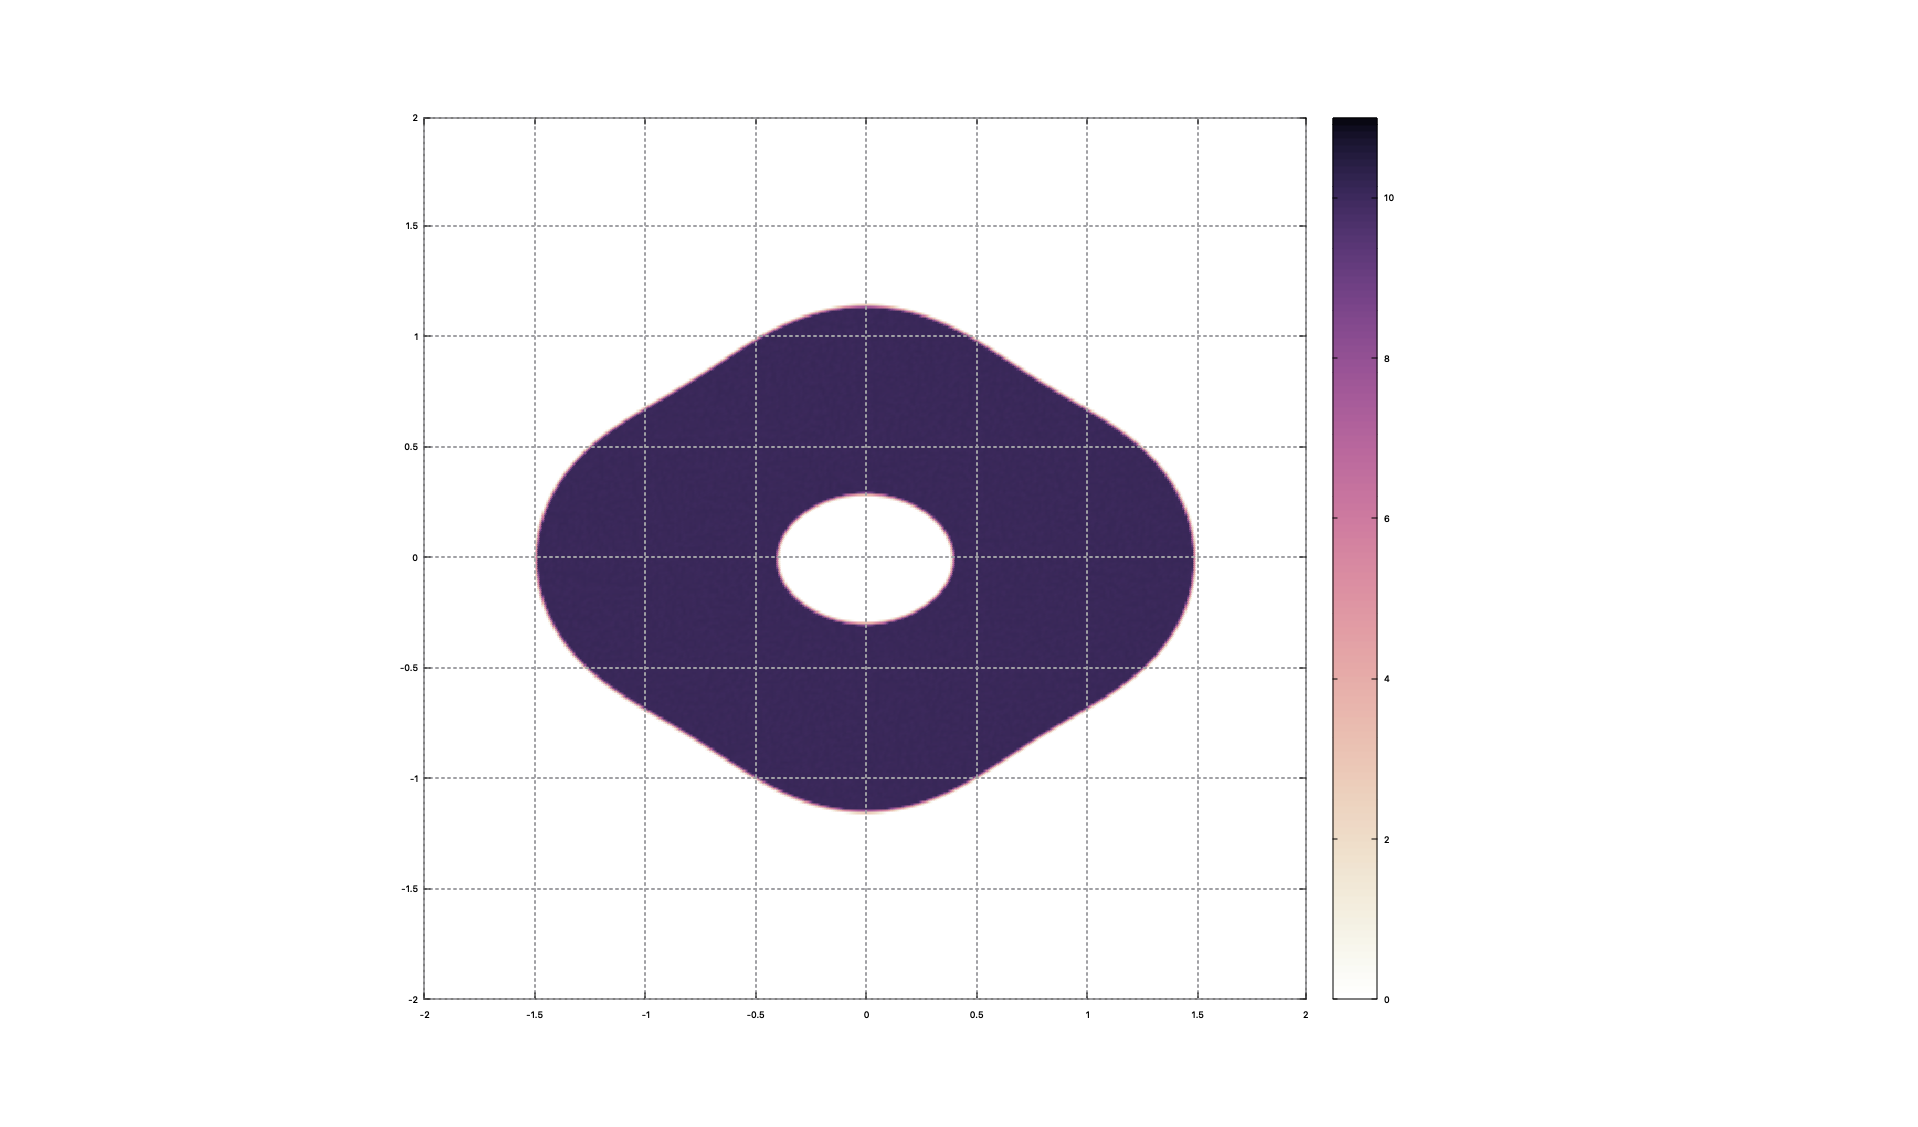
\includegraphics[width=4cm]{fig/PN300K100R10E2.png}
      % \captionsetup[figure]{labelformat=empty,labelsep=none}
      % \captionof{figure}{$a=10$}
    % \end{column}
    % \hspace{-1cm}
    % \begin{column}{0.38\columnwidth}
      % \centering
      % 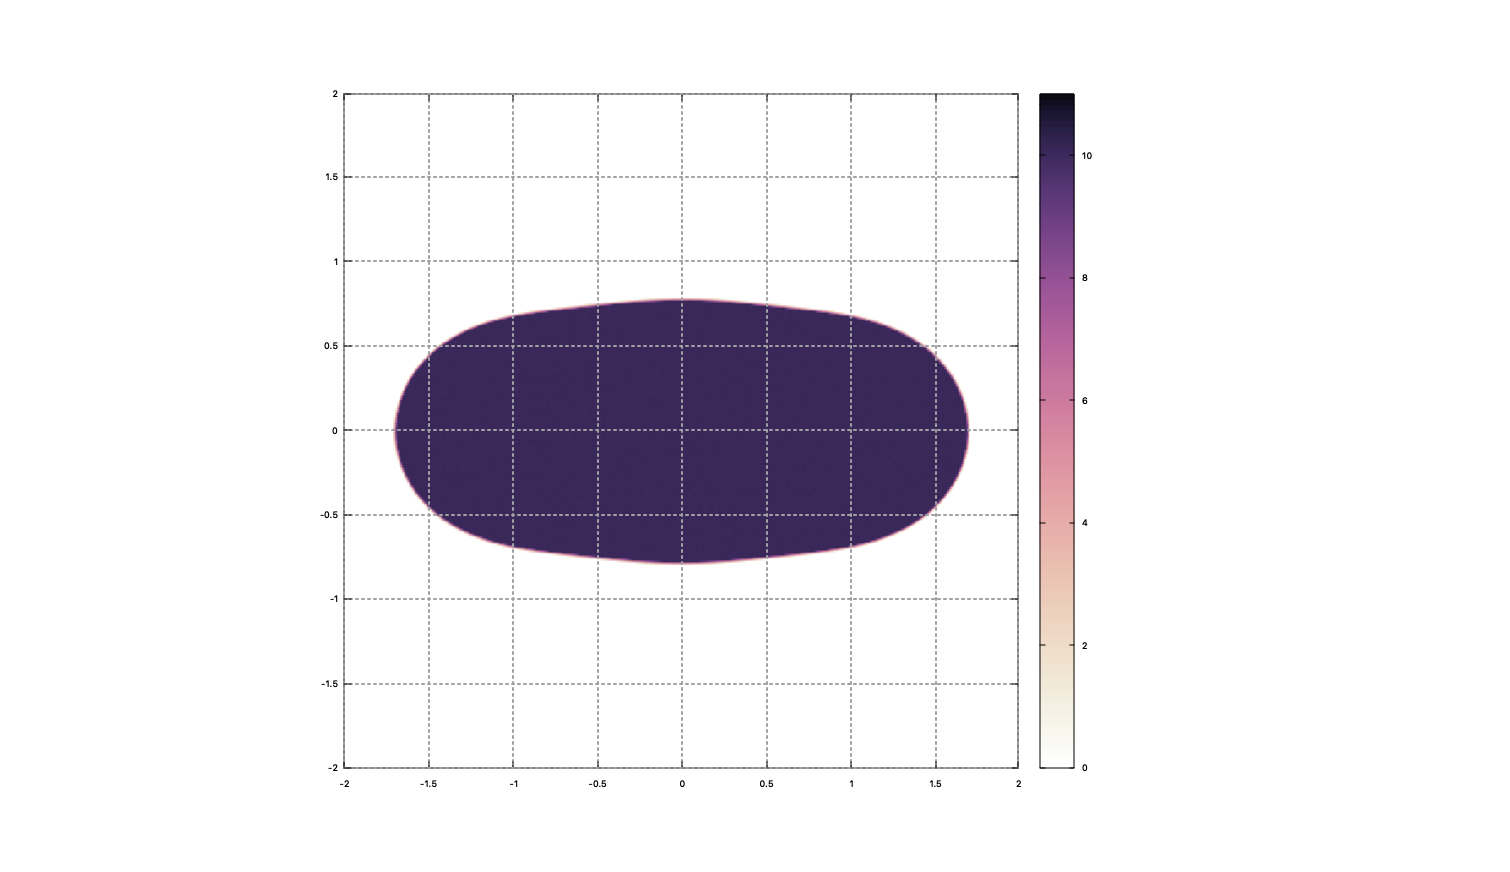
\includegraphics[width=4cm]{fig/PN300K100R30E2.png}
      % \captionsetup[figure]{labelformat=empty,labelsep=none}
      % \captionof{figure}{$a=30$}
    % \end{column}
  % \end{columns}

% \end{frame}


% % \begin{frame}{参考文献}
  % % \begin{thebibliography}{99}
    % % \bibitem{An}
    % % G.Anger, 
    % % \textit{Inverse Problems in Differential Equations},
    % % Plenum Press,
    % % 1990.
  
  
    % % \bibitem{Kr}
    % % R.Kress,
    % % \textit{Numerical Analysis},
    % % Springer,
    % % 1998.
  
    % % \bibitem{No}
    % % 野崎京三,
    % % 『原子時計をセンサーとした重力ポテンシャル計の可能性』,
    % % 応用地質技術年報,30号(2011),65-71.
  
    % % \bibitem{Sa}
    % % 佐々木晶,
    % % 『惑星内部構造』,
    % % 地震,61巻特集号(2009),285-296.
  
  
    % % \bibitem{Za}
    % % L.Zalcman,
    % % Some Inverse Problems of Potential Theory,
    % % \textit{Contemporary Mathematics}, Vol.63(1987), 337-339.
  
    % % \bibitem{Zi} 
    % % D.Zidarov, 
    % % \textit{Inverse Gravimetric Problem in Geoprospecting and Geodesy},
    % % Elsevier,
    % % 1990.
  % % \end{thebibliography}

% % \end{frame}

\end{document}
